\newpage
\criteria{Facilities and Infrastructure}

\subcriteria{The physical resources to deliver the curriculum, including equipment, material, and information technology, are shown to be sufficient.}

หลักสูตรใช้ทรัพยากรกายภาพและสิ่งสนับสนุนการเรียนรู้ของคณะและมหาวิทยาลัยในการจัดการเรียนการสอน โดยมีรายละเอียดดังนี้
\begin{enumerate}[label={},leftmargin=0cm]
\item {\bf 1. ห้องเรียนสำหรับการเรียนการสอน:}\\ \hspace*{1cm} มหาวิทยาลัยและคณะมีการจัดเตรียมห้องเรียนเพื่อรองรับการจัดการเรียนการสอนทั้งในรูปแบบ Onsite และ Online ที่พร้อมวัสดุอุปกรณ์เทคโนโลยีและอินเทอร์เน็ต ซึ่งในห้องเรียนแต่ละห้องจะประกอบด้วยอุปกรณ์ในการเรียนการสอน คอมพิวเตอร์ เครื่องฉายและฉาก ไมโครโฟน ลำโพง ที่พร้อมใช้งาน ในกรณีจัดการเรียนการสอนในรูปแบบ Online อาจารย์ผู้สอนสามารถใช้โปรแกรม Microsoft Teams เป็นโปรแกรมหลักในการจัดการเรียนการสอน  นอกจากนั้นระบบอินเทอร์เน็ตสามารถเชื่อมต่อได้ทุกห้องเรียนทั้งระบบ LAN และสัญญาณอินเทอร์เน็ตไร้สาย (WiFi) ทั้งนี้ในกรณีอุปกรณ์ต่าง ๆ ในห้องเรียนมีปัญหา อาจารย์สามารถติดต่อฝ่ายอาคารสถานที่ของคณะที่ดูแลรับผิดชอบผ่านทางโทรศัพท์ซึ่งมีการแจ้งหมายเลขติดต่อไว้ในทุกห้องเรียน เพื่อมาช่วยแก้ไขปัญหาให้แก่อาจารย์ได้ สำหรับห้องเรียนและห้องปฏิบัติการในความรับผิดชอบของหลักสูตรที่ใช้ในการจัดการเรียนการสอนในรายวิชาชีพและรายวิชาศึกษาทั่วไป (บางกลุ่ม) เป็นห้องเรียนจำนวน 3 ห้องและห้องปฏิบัติการจำนวน 3 ห้อง รายละเอียดดังตารางต่อไปนี้
\begin{center}
\begin{tabular}{|p{0.25\linewidth}|p{0.3\linewidth}|>{\centering}p{0.1\linewidth}|>{\centering}p{0.1\linewidth}|>{\centering\arraybackslash}p{0.1\linewidth}|}
\hline
\multicolumn{1}{|c|}{ชื่ออาคาร}&\multicolumn{1}{c}{ชื่อห้องเรียน/ห้องปฏิบัติการ}&\multicolumn{2}{|c|}{ประเภทห้อง} &ขนาด \\ \cline{3-4} 
&&ห้องเรียน&ห้องปฏิบัติการ&ความจุ (คน)\\\hline
อาคารเฉลิมพระเกียรติ ๖ รอบพระชนมพรรษา ชั้น 3& ห้องบรรยายรวม ST1- 301 &\checkmark&&80\\\hline
อาคารเฉลิมพระเกียรติ ๖ รอบพระชนมพรรษา ชั้น 3&ห้อง Research and Discussion ST1-908&&\checkmark&20\\\cline{2-5}
&ห้องปฏิบัติการคอมพิวเตอร์\newline ST1-905&&\checkmark&30\\\cline{2-5}
&ห้อง Smart Class Room\newline ST1-906&&\checkmark&60\\\cline{2-5}
&ห้องบรรยายรวม ST1-910&\checkmark&&40\\\cline{2-5}
&ห้องบรรยายรวม ST1-911&\checkmark&&40\\\hline
\end{tabular}
\end{center}

\noindent
{\bf หมายเหตุ}	สำหรับรายวิชาศึกษาทั่วไปหลักสูตรใช้ห้องเรียนที่อาคารเรียนรวมและปฏิบัติการ (รป. 13 ชั้น)

\begin{figure}
\begin{center}
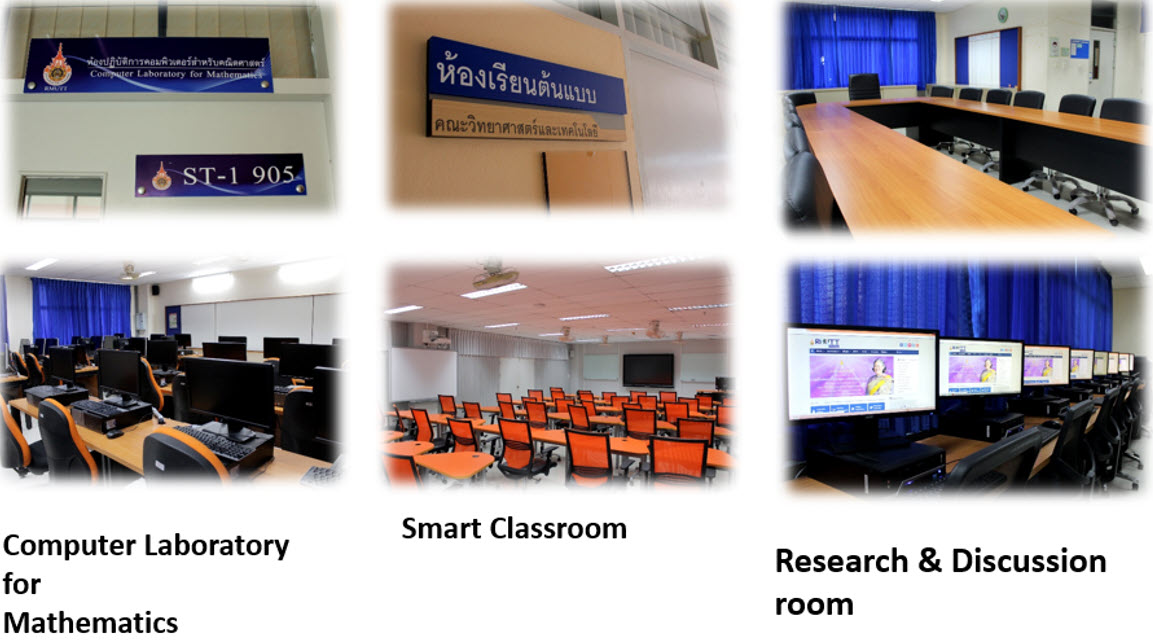
\includegraphics[width=0.9\textwidth]{Pic7.1-1.jpg}\\
\caption{ห้องปฏิบัติการ ST1-905 ST1-906 และ ST1-908}
\end{center}
\end{figure}
\newpage
\item {\bf 2. ห้องสมุด:}\\ {\bf $\bullet$ ห้องสมุดของมหาวิทยาลัย}\\
\hspace*{1cm} มีให้บริการหนังสือ วารสาร สื่อวิดีทัศน์ และอื่น ๆ วารสารเฉพาะสำหรับหลักสูตร e-Databases e-Theses ระบบสืบค้นข้อมูลทรัพยากรห้องสมุดผ่านระบบห้องสมุดอัตโนมัติ (Web OPAC) IT-Zone บริการสื่ออิเล็กทรอนิกส์ Edutainment ZONE ห้อง Boardgame ห้อง Mini Theater บริการจองห้องออนไลน์ บริการวารสาร นิตยสาร หนังสือพิมพ์ บริการด้านภาษา/โปรแกรมการฝึกปฏิบัติ/ทดสอบทางภาษา (SPEEXX (CLT), Chiness Mandarin, Sanako, ASEAN Language Learning) โดยห้องสมุดมหาวิทยาลัยมีพื้นที่ใช้สอย 20,000 ตารางเมตร มีหนังสือรวม 134,538 เล่ม แบ่งเป็นหนังสือทั่วไปภาษาไทย 86,159 เล่ม หนังสือทั่วไปภาษาอังกฤษ 19,906 เล่ม วิทยานิพนธ์จำนวน 4,853 เล่ม งานวิจัย 5,161 เล่ม  e-Book 5 ฐานข้อมูล จำนวน 29,107 เล่ม วารสาร 12 วารสาร โซนให้บริการชั้น 1 มีคอมพิวเตอร์ให้บริการ 84 เครื่อง  โซนให้บริการชั้น 3 มีคอมพิวเตอร์ให้บริการ 45 เครื่อง 
\begin{figure}[h!]
	\begin{center}
		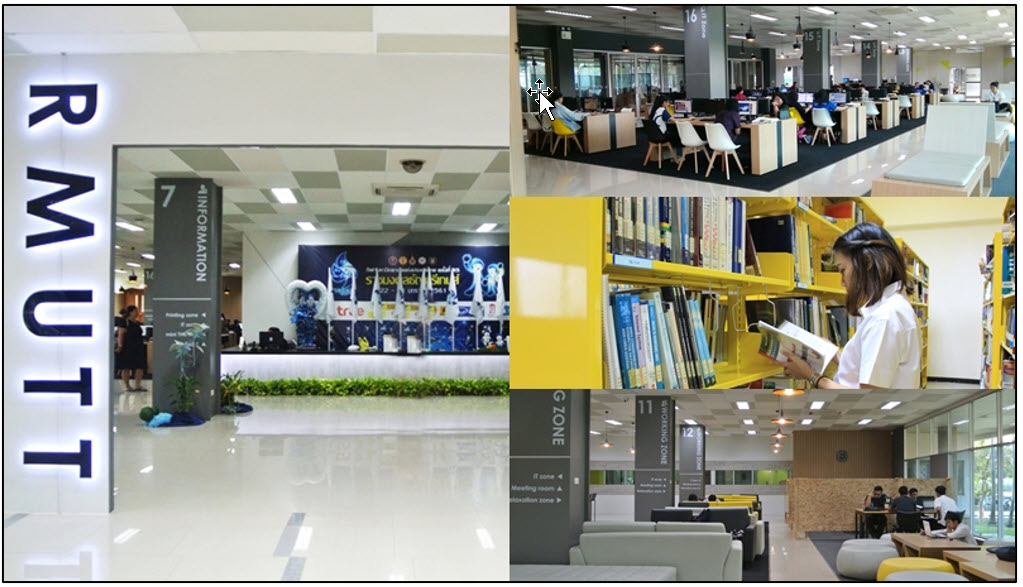
\includegraphics[width=0.8\textwidth]{Pic7.1-2.jpg}\\[0.2cm]
		\caption{ห้องสมุดของมหาวิทยาลัย}
	\end{center}
\end{figure}

\newpage
{\bf $\bullet$ ห้องสมุดคณะวิทยาศาสตร์และเทคโนโลยี มทร.ธัญบุรี}\\
\hspace*{1cm} มีบริการยืมคืนหนังสือเฉพาะทางด้านวิทยาศาสตร์และเทคโนโลยีสำหรับนักศึกษาในสาขาวิชาต่าง ๆ (เป็นหนังสือภาษาไทย จำนวน 6,828 เล่ม หนังสือภาษาอังกฤษ จำนวน 1,076 เล่ม) บริการห้อง Discussion Room จำนวน 10 ที่นั่ง ณ ชั้น 4 ห้องสมุด คณะวิทยาศาสตร์และเทคโนโลยี มทร.ธัญบุรี บริการตอบคำถามและช่วยค้นคว้า
\begin{figure}[h!]
	\begin{center}
		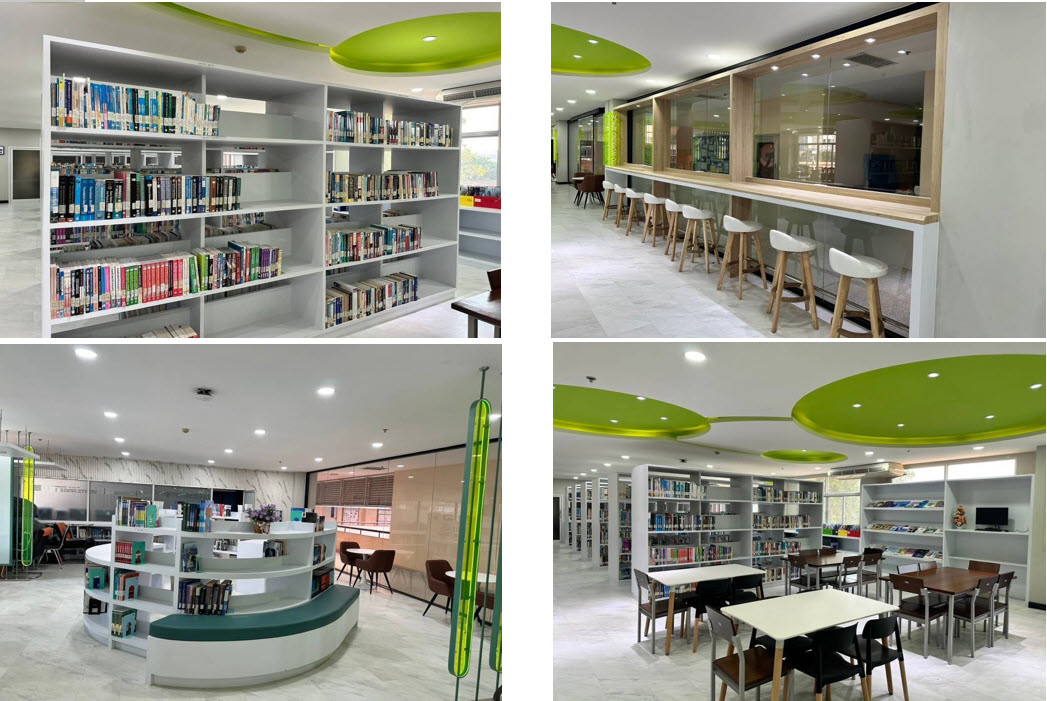
\includegraphics[width=0.8\textwidth]{Pic7.1-3.jpg}\\
		\caption{ห้องสมุดของคณะวิทยาศาสตร์และเทคโนโลยี}
	\end{center}
    \end{figure}
\\
ในส่วนของสาขาวิชามีหนังสือเฉพาะทางด้านคณิตศาสตร์  รวมทั้งเล่มโครงงานวิจัยและเล่มรายงานถอดบทเรียนรายวิชาสัมมนาของนักศึกษารุ่นพี่ สำหรับให้บริการนักศึกษา ที่ห้อง ST1-302 และห้อง ST1-908 
\begin{figure}[h!]
	\begin{center}
		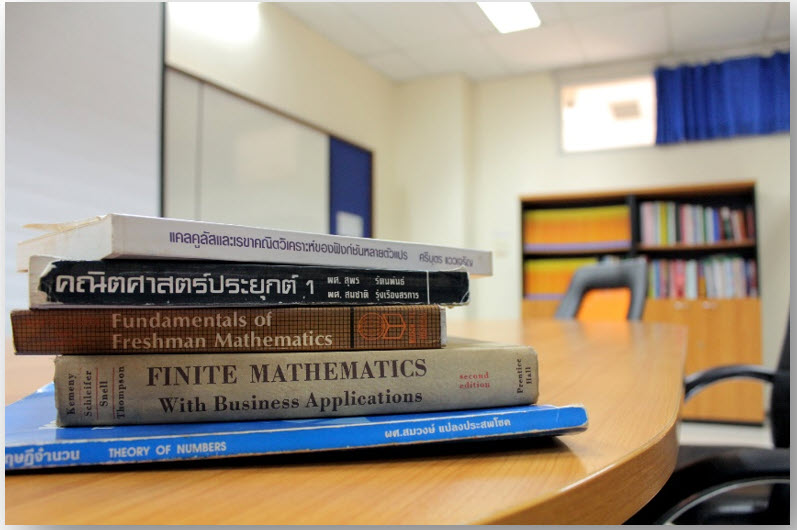
\includegraphics[width=0.8\textwidth]{Pic7.1-4.jpg}\\
		\caption{ห้องสมุดสาขาวิชาคณิตศาสตร์}
	\end{center}
\end{figure}

\end{enumerate}
\begin{doclist}
	\docitem{ห้องเรียนห้องปฏิบัติการของสาขาวิชา}
	\docitem{ภาพถ่ายห้องสมุดมหาวิทยาลัย ห้องสมุดคณะ ห้องสมุดสาขาวิชา}
\end{doclist}
%%%%%%%%%%%%%%%%%%%% 7.2 %%%%%%%%%%%%%%%
\subcriteria{The laboratories and equipment are shown to be up-to-date, readily available, and effectively deployed.}

สาขาวิชาคณิตศาสตร์ประยุกต์มีห้องปฏิบัติการคอมพิวเตอร์ในความรับผิดชอบจำนวน 1 ห้อง ได้แก่ ห้องปฏิบัติการ ST1-905 ความจุ 30 ที่นั่ง สำหรับให้บริการกับนักศึกษาที่เรียนในรายวิชาชีพ ของหลักสูตรฯ และรายวิชาชีพบางรายวิชาของหลักสูตรอื่นภายในคณะฯ ในห้องปฏิบัติการมีการลงโปรแกรมสำเร็จรูปที่จำเป็นสำหรับนักศึกษาสาขาวิชาคณิตศาสตร์ประยุกต์ เช่น MINITAB  SPSS โปรแกรมฟรี ที่เป็น open source เช่น โปรแกรม R  โปรแกรม Wx Maxima และ โปรแกรม Python เป็นต้น และมีการ update version ของโปรแกรมคอมพิวเตอร์อยู่เสมอเพื่อประโยชน์ในการใช้งานของอาจารย์และนักศึกษา โดยสาขาวิชามีเจ้าหน้าที่ห้องปฏิบัติการคอมพิวเตอร์ 1 คน ที่ดูแลและอำนวยความสะดวกให้กับนักศึกษาและอาจารย์ 

ในปีการศึกษา 2567 หลักสูตรได้รับจัดสรรงบประมาณจำนวน 92,750 บาท เพื่อใช้จัดซื้อวัสดุในการจัดการเรียนการสอนและปรับปรุงวัสดุต่าง ๆ ในห้องปฏิบัติการให้มีความพร้อมในการจัดการเรียนการสอนอยู่เสมอ นอกจากนี้ทางหลักสูตรมีการวางแผนปรับปรุงห้องปฎิบัติการโดยส่งคำเสนอของบประมาณรายจ่ายประจำปีงบประมาณ พ.ศ.2569 ในส่วนของครุภัณฑ์ไว้แล้ว



\begin{doclist}
	\docitem{ห้องปฏิบัติการของสาขาวิชา}
\end{doclist}

%%%%%%%%%%%%% 7.3 %%%%%%%%%%%%%
\subcriteria{A digital library is shown to be set-up, in keeping with progress in information and communication technology.}

หลักสูตรวิทยาศาสตรบัณฑิต สาขาวิชาคณิตศาสตร์ประยุกต์ ใช้ทรัพยากรด้านห้องสมุดดิจิทัลของ
มหาวิทยาลัย ซึ่งรับผิดชอบโดย สำนักวิทยบริการและเทคโนโลยีสารสนเทศ (สวส.) ที่ให้บริการฐานข้อมูลหนังสืออิเล็กทรอนิกส์ (e-Book) สำหรับนักศึกษา คณาจารย์ นักวิจัย และบุคลากรของมหาวิทยาลัยเทคโนโลยีราชมงคลธัญบุรี เพื่อการสืบค้นและการใช้งานฐานข้อมูลหนังสืออิเล็กทรอนิกส์สามารถเข้าถึงข้อมูลสารสนเทศตลอดจนเอกสารฉบับเต็มได้ ซึ่งบริการต่าง ๆ ประกอบไปด้วย
\begin{enumerate}
\item ฐานข้อมูลอิเล็กทรอนิกส์์เพื่อการสืบค้น เป็นการให้บริการฐานข้อมูล
อิเล็กทรอนิกส์ออนไลน์ทั้งในประเทศและต่างประเทศ เพื่อให้บริการแก่นักศึกษา อาจารย์ บุคลากร และนักวิจัยของมหาวิทยาลัย ให้สามารถใช้ทรัพยากรและเข้าถึงข้อมูลสารสนเทศเอกสารฉบับเต็มได้สะดวก รวดเร็ว ผ่านเครือข่ายสารสนเทศของมหาวิทยาลัย  ซึ่งประกอบไปด้วย 2 ส่วนคือ
 \begin{figure}[H]
 	\begin{center}
 		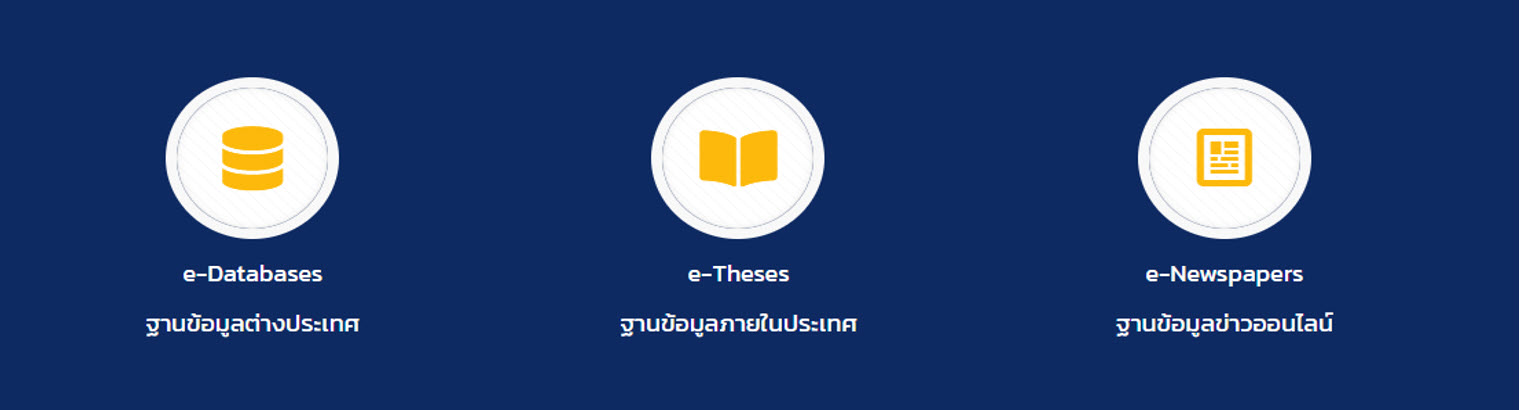
\includegraphics[width=0.65\textwidth]{Pic7.3-1.jpg}\\
 		%\caption{ห้องสมุดสาขาวิชาคณิตศาสตร์}
 	\end{center}
 \end{figure}
\begin{itemize}
	\item e-Databases เป็นฐานข้อมูลอิเล็กทรอนิกส์ออนไลน์ต่างประเทศ สนับสนุนโดยสำนักปลัดกระทรวงการอุดมศึกษา วิทยาศาสตร์ วิจัยและนวัตกรรม (อว.) ซึ่งฐานข้อมูลที่ให้บริการประกอบด้วย ฐานข้อมูลอ้างอิง (Reference Database) จำนวน 9 ฐานข้อมูล ที่เกี่ยวกับฐานข้อมูลวารสารอิเล็กทรอนิกส์ในสาขาวิชาต่าง ๆ รวมถึงฐานข้อมูลออนไลน์ที่บอกรับโดย สำนักวิทยบริการและเทคโนโลยีสารนิเทศ มทร.ธัญบุรี
	 \begin{figure}[H]
		\begin{center}
			\hspace*{2.2cm}
			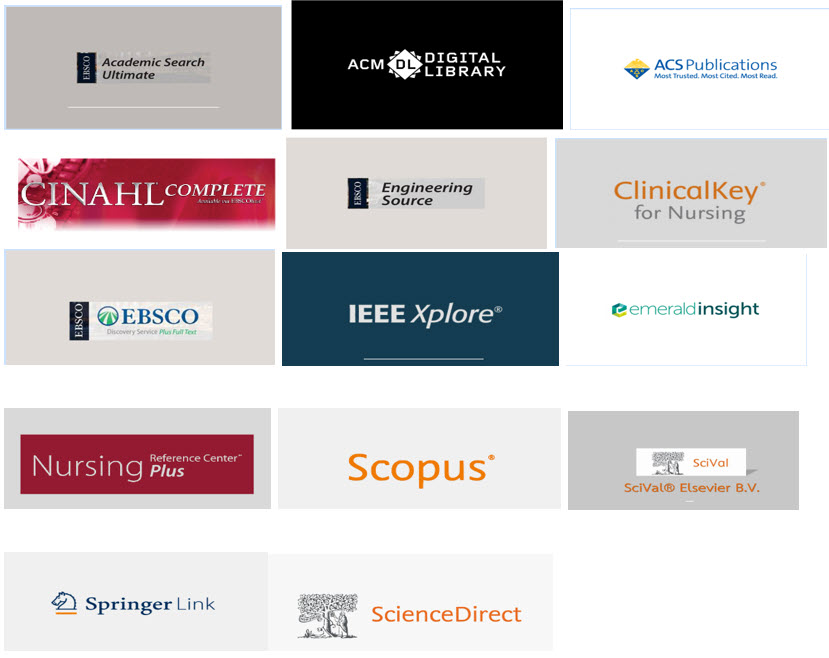
\includegraphics[width=0.8\textwidth]{Pic7.3-2.jpg}\\
			\caption{e-Databases ของห้องสมุดดิจิทัล RMUTT}
		\end{center}
	\end{figure}
	\item e-Theses เป็นการให้บริการฐานข้อมูลอิเล็กทรอนิกส์ออนไลน์ภายในประเทศ สำหรับสืบค้น
	ผลงานทางวิชาการของมหาวิทยาลัยภายในประเทศไทย และผลงานทางวิชาการของมหาวิทยาลัยเทคโนโลยีราชมงคลธัญบุรี ซึ่งประกอบด้วย งานวิจัย วิทยานิพนธ์ บทความวิชาการ และเอกสารเผยแพร่อื่น ๆ
\end{itemize}
\item บริการด้านภาษา เป็นการบริการโปรแกรมสำหรับฝึกทักษะทางด้านภาษา ทั้งทักษะภาษาอังกฤษ 
ภาษาจีน รวมถึงภาษาอาเซียน ซึ่งแต่ละโปรแกรมมุ่งเน้นให้ผู้รับบริการมีการพัฒนาทักษะการฟัง การพูด การอ่าน และคำศัพท์ เพื่อประยุกต์ใช้ในชีวิตประจำวัน การเรียนและการทำงานได้
	 \begin{figure}[H]
	\begin{center}
		\hspace*{1.5cm}
		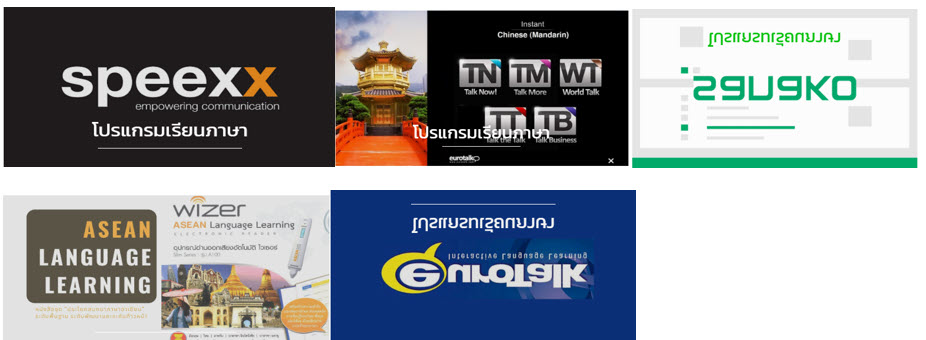
\includegraphics[width=0.8\textwidth]{Pic7.3-3.jpg}\\
		\caption{บริการด้านภาษา}
	\end{center}
\end{figure}
\item มีระบบ D-Learn @RMUTT เป็นระบบจัดการเรียนการสอนในระบบออนไลน์ให้มีบรรยากาศ
เหมือนการเรียนในห้องเรียน หรือเรียกว่า LMS (Learning Management System) นักศึกษา อาจารย์ หรือบุคลากรของมหาวิทยาลัยสามารถใช้งานระบบ D-Learn เพื่อจัดการเรียนการสอนได้ โดยอาจารย์สามารถจัดการรายวิชาของตนเองได้ เช่น การกำหนดบทเรียนและสื่อการสอน การกำหนดงานที่ได้รับมอบหมาย การทำแบบทดสอบ เป็นต้น รวมถึงนักศึกษาสามารถเข้าเรียนออนไลน์ได้ตลอดเวลา ซึ่งเหมาะกับการเรียนแบบ Flipped Classroom รวมถึงทำงานร่วมกับเครื่องมือติดต่อสื่อสารสำหรับประชุมออนไลน์ระหว่างอาจารย์และนักศึกษาได้
\item ให้บริการการตั้งค่าการเชื่อมต่อเครือข่ายมหาวิทยาลัยฯ (VPN) เพื่อ Remote Desktop 
Connection, ERP หรือ การสืบค้นงานวิจัย  VPN-RMUTT เป็นระบบเครือข่ายในมหาวิทยาลัยที่อนุญาตให้คณาจารย์ บุคลากรและนักศึกษาของมหาวิทยาลัย ที่อยู่นอกสถานที่สามารถเชื่อมต่อเข้ามาในเครือข่ายส่วนตัวของมหาวิทยาลัย เสมือนว่าอยู่ในเครือข่ายเดียวกับมหาวิทยาลัย เพื่อให้ง่ายต่อการทำงานต่าง ๆ ไม่ว่าจะเป็นการเข้าใช้ Remote Desktop Connection, ERP, การสืบค้นงานวิจัย โดยการเข้าใช้งานต้องมี ชื่อผู้ใช้และรหัสผ่าน ซึ่งเป็นชุดเดียวกับการ Login เข้าใช้งานเครือข่ายอินเทอร์เน็ต WiFi ของมหาวิทยาลัย


\end{enumerate}
\begin{doclist}
	\docitem{เว็บไซต์ห้องสมุดมหาวิทยาลัย\newline https://www.library.rmutt.ac.th}
\end{doclist}

%%%%%%%%%%%%% 7.4 %%%%%%%%%%%%%%%%
\subcriteria{The information technology systems are shown to be set up to meet the needs of staff and students.}

หลักสูตรใช้ระบบเทคโนโลยีสารสนเทศที่ตอบสนองความต้องการของบุคลากรและนักศึกษา 2 ส่วนด้วยกัน คือระบบเทคโนโลยีสารสนเทศของมหาวิทยาลัย และระบบเทคโนโลยีสารสนเทศที่คณะ ฯ พัฒนาขึ้นเอง
\begin{enumerate}
\item ระบบสารสนเทศของมหาวิทยาลัย\\
\textbf{- ระบบสารสนเทศที่สนับสนุนด้านการเรียนการสอน}
\begin{itemize} 
\item ระบบบริการการศึกษา (https://oreg.rmutt.ac.th) เป็นระบบสารสนเทศที่มีบทบาทอย่างมากสำหรับนักศึกษาและอาจารย์ที่ปรึกษา เพราะเป็นระบบที่นักศึกษาสามารถเข้ามาติดตามข่าวสารต่าง ๆ ค้นหารายวิชาเรียน ลงทะเบียนเรียนออนไลน์ ตรวจสอบผลการลงทะเบียนเรียนและพิมพ์ใบแจ้งยอดชำระเงิน ตรวจสอบตารางเรียนและตารางสอบ ตลอดจนตรวจสอบผลการเรียนของตนเอง การยื่นคำร้องออนไลน์ การถอนรายวิชาออนไลน์ และในส่วนของอาจารย์ที่ปรึกษา ระบบ OREG อำนวยความสะดวกในการติดตามความก้าวหน้าและผลการเรียนของนักศึกษาเพื่อที่ช่วยให้อาจารย์ที่ปรึกษาวางแผน ให้คำแนะนำ ตลอดจนช่วยแก้ไขปัญหาให้กับนักศึกษา
	 \begin{figure}[H]
	\begin{center}
		\hspace*{1.5cm}
		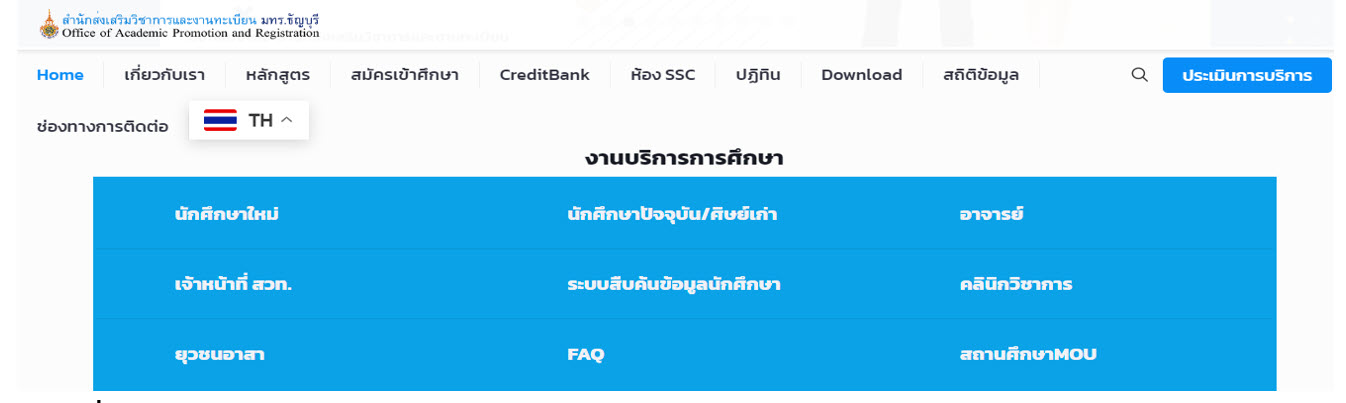
\includegraphics[width=0.65\textwidth]{Pic7.4-1.jpg}\\
		\caption{ระบบบริการการศึกษา}
	\end{center}
\end{figure}

\item ระบบรับสมัครนักศึกษาออนไลน์ เป็นระบบที่อำนวยความสะดวกให้นักเรียน มัธยมศึกษาตอนปลาย หรือผู้ต้องการเข้าศึกษาต่อสามารถดำเนินการสมัครเรียนและยื่นเอกสารได้จากทุกที่ทุกเวลา ซึ่งในระบบนี้ผู้สมัครเรียนสามารถตรวจสอบผลการสอบ ดำเนินการรายงานตัว ตรวจสอบสถานะการรายงานตัว พิมพ์ใบชำระเงิน
	 \begin{figure}[H]
	\begin{center}
		\hspace*{1.5cm}
		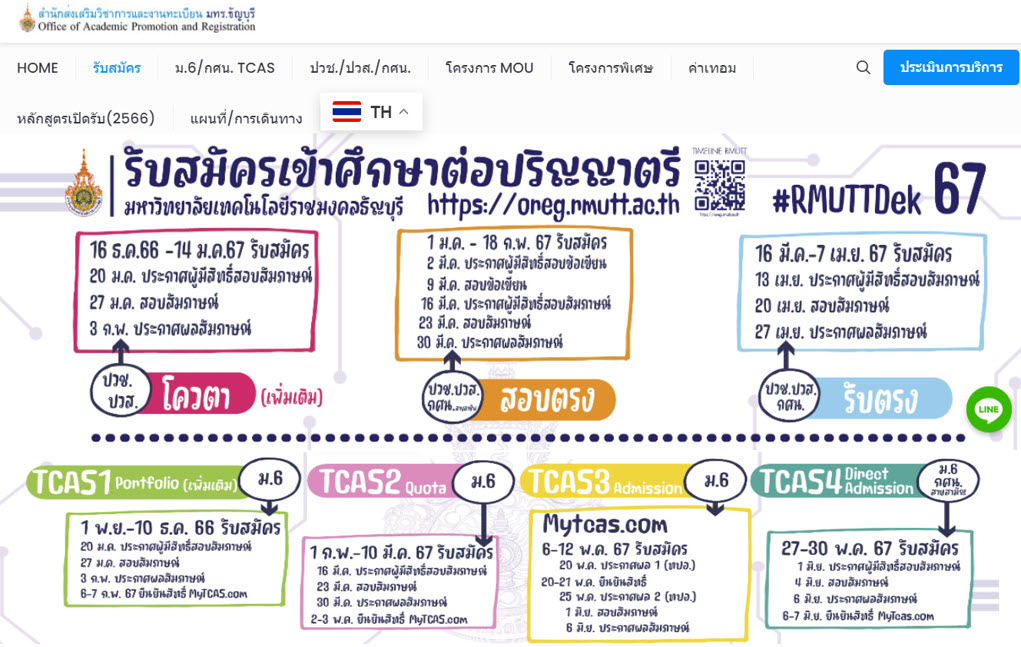
\includegraphics[width=0.7\textwidth]{Pic7.4-2.jpg}\\
		\caption{ระบบรับสมัครนักศึกษาออนไลน์}
	\end{center}
\end{figure}
\end{itemize}
\textbf{- ระบบสารสนเทศสนับสนุนด้านการวิจัย}
\begin{itemize}
\item ระบบข้อมูลสารสนเทศวิจัยและนวัตกรรม มทร.ธัญบุรี (https://urms.rmutt.ac.th/) ที่ช่วยในการติดตามและบริการจัดการงานวิจัยทั้งหมดจำนวน  3,796 โครงการ ทั้งงานวิจัยที่เป็นงบประมาณรายจ่าย งบประมาณรายได้ งบประมาณกองทุนส่งเสริมงานวิจัย และงบประมาณส่วนตัว ของทุกคณะ/หน่วยงาน ในมหาวิทยาลัย
	 \begin{figure}[H]
	\begin{center}
		\hspace*{1.5cm}
		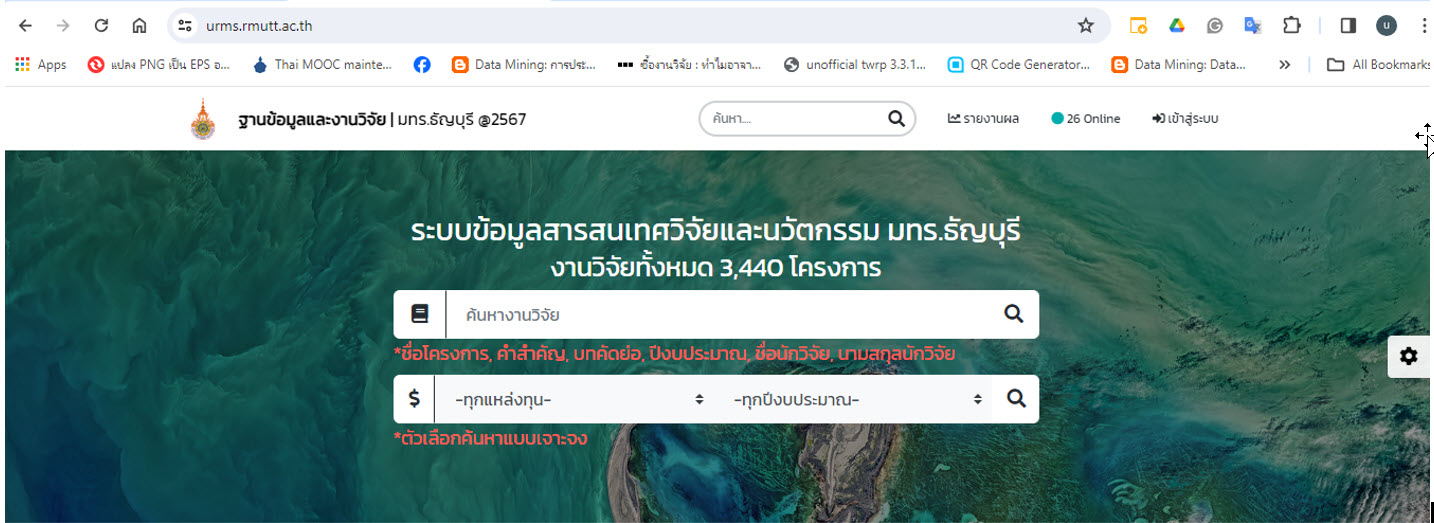
\includegraphics[width=0.7\textwidth]{Pic7.4-3.jpg}\\
\caption{ระบบข้อมูลสารสนเทศวิจัยและนวัตกรรม}
	\end{center}
\end{figure}
\end{itemize}
\textbf{- ระบบสารสนเทศเพื่อการบริหารจัดการ}
\begin{itemize}
	\item ระบบบุคลากรออนไลน์ (hr-online) 
	บุคลากรสามารถเข้าดูข้อมูลบุคลากรรายบุคคลประวัติการลาของบุคลากร ใบแจ้งเงินเดือน ปฏิทินการลงเวลา แจ้งผลการเลื่อนเงินเดือน เครื่องราชอิสริยาภรณ์ พิมพ์คำร้องขอแก้ไขข้อมูลประวัติส่วนตัว แสดงความคิดเห็น และสอบถามข้อมูล (ถาม-ตอบ) กราฟแสดงผลการประเมินเลื่อนเงินเดือนย้อนหลัง 5 ปี
	\item ระบบสำนักงานอิเล็กทรอนิกส์ (e-office) การบริหารจัดการเอกสารเข้า-ออก จดหมาย
	อิเล็กทรอนิกส์ การจัดเก็บเอกสาร แก้ไขเอกสาร งานเอกสารทางด้านบัญชี และการใช้ประโยชน์อื่น ๆ อีกมากมาย โดยอำนวยความสะดวกในเรื่องการลดขั้นตอน ลดระยะเวลา ลดการใช้ทรัพยากรกระดาษ (paperless) และอำนวยความสะดวกในการบริหารจัดการ การรับ-ส่งข้อมูลข่าวสาร มีการจัดเก็บเอกสารในลักษณะไฟล์ดิจิทัลอย่างเป็นระบบ มีความสะดวกรวดเร็ว และสามารถเข้าถึงและค้นหาข้อมูลได้ง่าย แม้ว่าผู้ปฏิบัติงานจะไม่อยู่ในสำนักงานก็สามารถเข้าถึงข้อมูลได้
	\item ระบบประชุมอิเล็กทรอนิกส์ (e-Meeting)
	\item ระบบจองห้องออนไลน์
\end{itemize}
\item ระบบสารสนเทศที่พัฒนาขึ้นเองโดยคณะวิทยาศาสตร์และเทคโนโลยี 
\begin{itemize}
	\item ระบบบริหารข้อมูลงานวิจัยและงานบริการวิชาการคณะวิทยาศาสตร์และเทคโนโลยี เพื่อบริหาร
	จัดการระบบบริหารข้อมูลงานวิจัยและงานบริการวิชาการ เพื่อเป็นแหล่งรวบรวมข้อมูลผลงานทางวิชาการ งานวิจัยตีพิมพ์ โครงการวิจัย งานวิจัยที่นำไปใช้ประโยชน์ นวัตกรรม ช่วยในการค้นคว้าอ้างอิง การรายงานผล ตอบโจทย์ยุทธศาสตร์ด้านงานวิจัยและบริการวิชาการของคณะและมหาวิทยาลัย
	\item 	ระบบจัดการข้อมูลการประเมินบุคลากรคณะวิทยาศาสตร์และเทคโนโลยีออนไลน์ เพื่อช่วยบริหาร
	จัดการเกี่ยวกับการประเมินผลการปฏิบัติราชการของบุคลากรสายวิชาการของคณะในทุกกลุ่ม ประกอบไปด้วย 
	\begin{itemize}
	\item พนักงานมหาวิทยาลัยวุฒิปริญญาเอก
	\item พนักงานมหาวิทยาลัยวุฒิปริญญาโท 
	\item ข้าราชการพลเรือน 
	\item ข้าราชการ (ที่เป็นผู้บริหาร)
	\item พนักงานมหาวิทยาลัยวุฒิปริญญาเอก (ที่เป็นผู้บริหาร) 
	\end{itemize}
\end{itemize}
\end{enumerate}

\begin{doclist}
	\docitem{ระบบสารสนเทศของมหาวิทยาลัย}
	\docitem{ระบบสารสนเทศที่พัฒนาขึ้นเองโดยคณะวิทยาศาสตร์และเทคโนโลยี}
\end{doclist}
%%%%%%%%%%% 7.5 %%%%%%%%%%%%%%%%%%%%%%%%%%
\subcriteria{The university is shown to provide a highly accessible computer and network infrastructure that enables the campus community to fully exploit information technology for teaching, research, service, and administration.}

หลักสูตรใช้ระบบโครงสร้างพื้นฐานด้านคอมพิวเตอร์และระบบเครือข่ายเทคโนโลยีสารสนเทศ ที่มีการจัดเตรียมและให้บริการโดยสำนักวิทยบริการและเทคโนโลยีสารสนเทศ (สวส.) โดยระบบดังกล่าวมีความทันสมัย เพียงพอ และพร้อมใช้ ตรงกับความต้องการของทั้งในด้านการเรียนการสอน การวิจัย การบริการวิชาการ และการบริหารจัดการ ซึ่งประกอบไปด้วย
\begin{enumerate}
	\item การใช้บริการเครือข่ายไร้สาย (WiFi RMUTT) มหาวิทยาลัยเทคโนโลยีราชมงคลธัญบุรี ทางสำนักวิทยบริการและเทคโนโลยีสารสนเทศได้ให้บริการครอบคลุมทั่วทุกจุดใน มทร.ธัญบุรี เช่น
	\begin{itemize}[label=-]
	\item  บริเวณสำนักวิทยบริการและเทคโนโลยีสารสนเทศ (อาคาร ICT, Training, iWork@RT, Library)
	\item อาคารเรียนตามคณะต่าง ๆ
	\item บ้านพักสวัสดิการ ข้าราชการ พนักงานมหาวิทยาลัย มทร.ธัญบุรี
	\item หอพักสวัสดิการนักศึกษา มทร.ธัญบุรี
	\item อาคารเรียนรวมและปฏิบัติการ
\end{itemize}
\hspace*{1cm}บุคลากรสามารถเข้าใช้บริการ Wifi@RMUTT ได้โดยใช้ Username : ประกอบด้วย ชื่อ
	ภาษาอังกฤษ ตามด้วยสัญลักษณ์ (\_) และตามด้วยอักษรตัวแรกของนามสกุลภาษาอังกฤษ เช่น ชื่อ Somsak Rmutt ในการกำหนด username จะกำหนดเป็น somsak\_r (ในกรณีนามสกุลตัวแรกซ้ำจะตามด้วยนามสกุลตัวแรกและตัวที่ 2 ของนามสกุล) Password : กำหนดเป็นตัวเลข 6 หลักท้ายจากรหัสบัตรประชาชน
	(โดยบุคลากรสามารถเปลี่ยน Password ได้ด้วยตนเองในภายหลัง) \\[0.2cm]
\hspace*{1cm}นักศึกษาสามารถเข้าใช้บริการ Wifi@RMUTT ได้โดยใช้ Username :  รหัสนักศึกษา 13 หลักโดยไม่ต้องใส่ขีด (-) Password : กำหนดเป็นตัวเลข 6 หลักท้ายจากรหัสบัตรประชาชน
(โดยนักศึกษาสามารถเปลี่ยน Password ได้ด้วยตนเองในภายหลัง)\\[0.2cm]
\hspace*{1cm}ในส่วนของคณะวิทยาศาสตร์และเทคโนโลยีมี 2 อาคารเรียน คือ อาคารเฉลิมพระเกียรติ ๖ รอบพระชนมพรรษา (อาคาร 9 ชั้น) และอาคารสถาบันวิจัยเคมี (อาคาร 4 ชั้น) โดยทุกชั้นของแต่ละอาคารมีจุดเชื่อมต่อสัญญาณ WiFi ทุกชั้น ทำให้สามารถใช้งานได้อย่างไม่ติดขัด \\[0.2cm]
\hspace*{1cm}นอกจากนี้ยังมีการให้บริการการใช้งาน ระบบ Backoffice กรณีที่ไม่ได้ตั้งค่า VPN สามารถทำการตั้งค่า VPN ได้ที่ http://www.ict.rmutt.ac.th/?p=2384  หรือนำเครื่องคอมพิวเตอร์ส่วนบุคคล (Notebook) มาให้เจ้าหน้าที่ที่ สวส. ดำเนินการตั้งค่าระบบ VPN \\[0.2cm]
\hspace*{1cm}โดยทางสำนักวิทยบริการฯ มีแนวทางจะให้ครอบคลุมทั่วทุกจุดใน มทร.ธัญบุรี เร็ว ๆ นี้
\item 	ในส่วนของคณะมีห้องปฏิบัติคอมพิวเตอร์จำนวน  16  ห้อง รวมจำนวนเครื่องคอมพิวเตอร์ที่ให้บริการนักศึกษา จำนวน 522 เครื่อง โดยมีรายละเอียดดังตารางต่อไปนี้ \\[0.2cm]
{\small
%\begin{table}[H]
	\begin{tabular}{|c|c|c|c|c|}
		\hline
		\textbf{ลำดับที่} & \textbf{สาขาวิชา}                                                                                                         & \textbf{ชั้น} & \textbf{ห้อง} & \textbf{จำนวนเครื่อง} \\ \hline
		1                 & -                                                                                                                         & 4             & IT\&SCI       & 20                    \\ \hline
		2                 & สาขาวิชาฟิสิกส์                                                                                                           & 7             & ST1-710       & 37                    \\ \hline
		3                 & \multirow{10}{*}{\begin{tabular}[c]{@{}c@{}}สาขาวิชาวิทยาการคอมพิวเตอร์ และ \\ สาขาวิชาเทคโนโลยีคอมพิวเตอร์\end{tabular}} & 8             & ST1-804       & 30                    \\ \cline{1-1} \cline{3-5} 
		4                 &                                                                                                                           & 8             & ST1-805       & 31                    \\ \cline{1-1} \cline{3-5} 
		5                 &                                                                                                                           & 8             & ST1-806       & 31                    \\ \cline{1-1} \cline{3-5} 
		6                 &                                                                                                                           & 8             & ST1-807       & 37                    \\ \cline{1-1} \cline{3-5} 
		7                 &                                                                                                                           & 8             & ST1-809       & 61                    \\ \cline{1-1} \cline{3-5} 
		8                 &                                                                                                                           & 8             & ST1-810       & 30                    \\ \cline{1-1} \cline{3-5} 
		9                 &                                                                                                                           & 8             & ST1-811       & 30                    \\ \cline{1-1} \cline{3-5} 
		10                &                                                                                                                           & 8             & ST1-812       & 31                    \\ \cline{1-1} \cline{3-5} 
		11                &                                                                                                                           & 8             & ST1-813       & 30                    \\ \cline{1-1} \cline{3-5} 
		12                &                                                                                                                           & 8             & ST1-814       & 31                    \\ \hline
		13                & \multirow{4}{*}{\begin{tabular}[c]{@{}c@{}}สาขาวิชาคณิตศาสตร์ และ \\ สาขาวิชาสถิติประยุกต์\end{tabular}}                  & 9             & ST1-904       & 32                    \\ \cline{1-1} \cline{3-5} 
		14                &                                                                                                                           & 9             & ST1-905       & 30                    \\ \cline{1-1} \cline{3-5} 
		15                &                                                                                                                           & 9             & ST1-912       & 36                    \\ \cline{1-1} \cline{3-5} 
		16                &                                                                                                                           & 9             & ST1-914       & 25                    \\ \hline
	\end{tabular}
}
\item สำนักวิทยบริการ ฯ มีบริการ IT zone ณ อาคารวิทยบริการ จัดพื้นที่ให้ผู้ใช้บริการสามารถใช้คอมพิวเตอร์สำหรับค้นหาข้อมูลทางวิชาการ โปรแกรมการทำงาน เรียนออนไลน์ และนันทนาการ  ผู้ใช้บริการสามารถใช้บริการได้โดยต้องมี Username และ Password WiFi RMUTT  มีบริการเครื่องคอมพิวเตอร์ สำหรับค้นหาข้อมูลทางวิชาการ โปรแกรมการทำงาน เรียนออนไลน์ และนันทนาการ  รวมทั้งหมดจำนวน 84 เครื่อง  เครื่องคอมพิวเตอร์รองรับการสั่ง Print เอกสารออนไลน์ ได้จำนวน 64 เครื่อง
\item สำนักวิทยบริการ ฯ มีการพัฒนาระบบสมุดบันทึกกิจกรรม (Activity RMUTT) สำหรับนักศึกษา
\item สำนักวิทยบริการ ฯ ให้บริการจองห้อง ประกอบไปด้วย อาคารเรียนรวมและปฏิบัติการ (Central Building)  ห้อง Discussion Room 4 - 15 ที่นั่ง ห้องปฏิบัติการ Computer 40 - 80 ที่นั่ง  ห้อง Smart Classroom ห้อง Classroom 40 - 120 ที่นั่ง  ห้องประชุม/สัมมนา 100 ที่นั่ง
\item สำนักวิทยบริการ ฯ ให้บริการระบบห้องเรียนออนไลน์ D-Learn @RMUTT สำหรับอาจารย์ผู้สอนเพื่อจัดการเรียนการสอนในระบบออนไลน์ให้มีบรรยากาศเหมือนการเรียนในห้องเรียน โดยนักศึกษา อาจารย์ หรือบุคลากรของมหาวิทยาลัยที่สนใจสามารถใช้งานระบบ D-Learn เพื่อจัดการเรียนการสอน อาจารย์สามารถจัดการรายวิชาของตนเองได้ เช่น การกำหนดบทเรียนและสื่อการสอน การกำหนดงานมอบหมาย การทำแบบทดสอบ เป็นต้น รวมถึงนักศึกษาสามารถเข้าเรียนออนไลน์ได้ตลอดเวลา ซึ่งเหมาะกับการเรียนแบบ Flipped Classroom รวมถึงทำงานร่วมกับเครื่องมือติดต่อสื่อสารสำหรับประชุมออนไลน์ระหว่างอาจารย์และนักศึกษาได้   การจัดการเรียนการสอนออนไลน์ ผ่านระบบ Microsoft Teams
\end{enumerate}

\begin{doclist}
	\docitem{ข้อมูลของโครงสร้างพื้นฐานด้านคอมพิวเตอร์และเครือข่ายพื้นฐานที่จัดหาโดยคณะและมหาวิทยาลัย}
\end{doclist}


%%%%%%%%%%% 7.6 %%%%%%%%%%%%%%%%%%%%%%%%%%
\subcriteria{The environmental, health, and safety standards and access for people with special needs are shown to be defined and implemented.}

นักศึกษาของหลักสูตรส่วนใหญ่เรียนในอาคารเรียน อาคารเฉลิมพระเกียรติ ๖ รอบพระชนมพรรษา คณะวิทยาศาสตร์และเทคโนโลยี 9 ชั้น  (ห้องเรียนและห้องปฏิบัติการอยู่บริเวณชั้น 9) เป็นส่วนใหญ่  เนื่องจากเป็นตึกสูงดังนั้นองค์ประกอบด้านความปลอดภัยที่ต้องมีคือ ข้อกำหนดด้านความปลอดภัยในอาคารสูง โดยมีกฎหมายที่เกี่ยวข้องคือ
กฎกระทรวงฉบับที่ 33 (พ.ศ.2535) ฉบับที่ 47 (พ.ศ.2540) ฉบับที่ 48 (พ.ศ.2540) และฉบับที่ 50 (พ.ศ.2540) ออกตามความในพระราชบัญญัติควบคุมอาคาร พ.ศ.2522

{\bf ด้านความปลอดภัย}

การดูแลระบบไฟฟ้าและดับเพลิง เป็นหน้าที่ของงานอาคารสถานที่คณะ มีการจัดเตรียมอุปกรณ์ดับเพลิงที่พร้อมใช้งานในทุกชั้นของอาคาร มีการตรวจสอบอุปกรณ์ถังดับเพลิงสม่ำเสมอ ปีการศึกษาละ 1 ครั้งและมีการจัดการฝึกซ้อมอพยพหนีไฟ ปีการศึกษาละ 1 ครั้ง

ในทุก ๆ ห้องเรียนห้องปฏิบัติการ จะมีระบบรักษาความปลอดภัย ได้แก่
\begin{enumerate}
	\item มีระบบ smoke detector หากพบกลุ่มควันภายในห้องจะมีการแจ้งเตือนไปที่ห้องของเจ้าหน้าที่อาคารสถานที่ของคณะ
	\item มีระบบหัวดับเพลิงติดอยู่บนฝ้าเพดานเมื่อเจอความร้อนจะปล่อยน้ำในท่อออกมาเพื่อระงับการเกิดเพลิงไหม้
	\item มีตู้ควบคุมระบบไฟฟ้าเพื่อตัดไฟเมื่อเกิดเพลิงไหม้
\end{enumerate}

นอกจากนั้นยังมีการออกกฎข้อปฏิบัติในการใช้ห้องปฏิบัติการคอมพิวเตอร์ โดยมีป้ายเตือนนักศึกษา หลังเลิกใช้เครื่องคอมพิวเตอร์ในห้องปฏิบัติการควรปิดเครื่องคอมพิวเตอร์ให้เรียบร้อยก่อนออกจากห้อง เพื่อป้องกันปัญหาด้านความร้อนของอุปกรณ์คอมพิวเตอร์

{\bf ด้านสุขภาพ}

ในแต่ละปีจะมีการตรวจสุขภาพประจำปีให้กับนักศึกษาและบุคลากรทุกคน และมหาวิทยาลัยได้ดำเนินการจัดทำประกันอุบัติเหตุให้กับนักศึกษาและบุคลากรทุกคนทุกปี ตลอดจนมีการตรวจสารเสพติดในนักศึกษาเพื่อป้องกันปัญหาสารเสพติดในสถานศึกษา มีกิจกรรมอบรมให้ความรู้เกี่ยวกับอันตรายของยาเสพติด/บุหรี่ ซึ่งดำเนินการโดยกองพัฒนานักศึกษา

ด้านสาธารณูปโภคและการรักษาความปลอดภัย
คณะมีการจ้างแม่บ้านในการดูแลทำความสะอาดกำจัดขยะมูลฝอยในหน่วยงานทุกวัน และจัดกิจกรรม 5ส ภายในหน่วยงานและมีการประกวดกิจกรรม 5ส ในทุก ๆ ปี ในแต่ละชั้นของตึกมีน้ำดื่มสะอาดให้บริการกับนักศึกษา
ในส่วนการเข้าถึงของบุคคลที่มีความต้องการพิเศษ (Access for People with special needs) มีการดำเนินการ เช่น จัดให้มีทางลาดขึ้นลงอาคาร จัดให้มีลิฟต์หรือทางลาดที่ผู้พิการหรือทุพพลภาพและคนชราใช้ได้  จัดให้มีห้องน้ำสำหรับผู้พิการหรือทุพพลภาพ เป็นต้น


\begin{doclist}
	\docitem{ข้อมูลมาตรฐานด้านความปลอดภัย/สิ่งแวดล้อม }
	\docitem{ข้อมูลมาตรฐานของผู้ที่มีความต้องการพิเศษ }
\end{doclist}

%%%%%%%%%%% 7.7 %%%%%%%%%%%%%%%%%%%%%%%%%%
\subcriteria{The university is shown to provide a physical, social, and psychological environment that is conducive for education, research, and personal well-being.}
\begin{enumerate}
\item {\bf ด้านสิ่งแวดล้อมทางกายภาพ}\\ 
กองอาคารสถานที่ของมหาวิทยาลัย และงานอาคารสถานที่คณะ เป็นผู้รับผิดชอบการจัดการอาคารสถานที่ ให้มีความพร้อมใช้ เพียงพอต่อจำนวนนักศึกษา โดยมีการทบทวนการจัดสิ่งอำนวยความสะดวกของนักศึกษาทุกสิ้นปีการศึกษา สิ่งอำนวยความสะดวกด้านสิ่งแวดล้อมทางกายภาพประกอบไปด้วย
\begin{enumerate}[label=\arabic*), leftmargin=1.2cm]
\item อาคารเฉลิมพระเกียรติ ๖ รอบพระชนมพรรษา คณะวิทยาศาสตร์และเทคโนโลยี 9 ชั้น  ซึ่งประกอบไปด้วยห้องเรียน ห้องปฏิบัติการ และพื้นที่การเรียนรู้ Learning Space สำหรับนักศึกษาในการศึกษาค้นคว้าความรู้ด้วยตนเองและทำวิจัย 
\item ห้องอเนกประสงค์ ชั้น 1 (นลินวิทย์) เพื่อใช้จัดกิจกรรม หรือเวทีการประกวดต่าง ๆ หรือใช้ซ้อมการแสดง 
\item พื้นที่บริเวณลานปาล์มและชั้น 1 ของคณะที่ปรับทัศนียภาพเป็นลักษณะสวนหย่อม เพื่อใช้พักผ่อนหย่อนใจ 
\item ชั้น 1 อาคารเฉลิมพระเกียรติ ๖ รอบพระชนมพรรษา คณะวิทยาศาสตร์และเทคโนโลยีมีพื้นที่ให้นักศึกษานั่งทำกิจกรรมหรือรอเรียน
\item มีสนามกีฬาบริการให้กับนักศึกษา
\item มีห้องพยาบาลและรถพยาบาล 
\item ที่จอดรถบริเวณรอบคณะ
\item มีเครื่องถ่ายเอกสาร 
\item มีรถไฟฟ้ารับส่งภายในพื้นที่ มทร.ธัญบุรี และสกู๊ตเตอร์ไฟฟ้า พลังงานสะอาด ไม่ต้องเติมน้ำมัน
 รักษาสิ่งแวดล้อม
\end{enumerate}
\item {\bf ด้านสิ่งแวดล้อมทางสังคม}\\ 
กองพัฒนานักศึกษาเป็นผู้รับผิดชอบการจัดชมรม จัดกิจกรรมพัฒนาศักยภาพของนักศึกษาในภาพรวมของมหาวิทยาลัย รวมถึงคณะดำเนินการจัดโครงการพัฒนาศักยภาพของนักศึกษาในภาพรวมของคณะ ตัวอย่างของการจัดหาสิ่งแวดล้อมทางสังคม เช่น 
\begin{enumerate}[label=\arabic*), leftmargin=1.2cm]
\item กิจกรรมพิเศษนอกหลักสูตร :  มีการจัดกิจกรรมพิเศษนอกหลักสูตรต่าง ๆ ให้แก่ นักศึกษาสามารถเข้าร่วมกิจกรรม เพื่อเป็นการพัฒนาและเสริมสร้างทักษะด้านต่าง ๆ เช่น พิธีไหว้ครู โครงการปฐมนิเทศนักศึกษาใหม่ โครงการปัจฉิมนิเทศนักศึกษา เป็นต้น
\item กิจกรรมชมรม : มีการสนับสนุนการจัดตั้งชมรมแก่นักศึกษา เช่น ชมรม Green University 
\item สโมสรนักศึกษา : มีการจัดตั้งกรรมกาบริหารรสโมสรนักศึกษา ซึ่งมีตัวแทนจากนักศึกษาแต่ละสาขาร่วมกันวางแผนการจัดกิจกรรมที่นักศึกษาสนใจ
\item การจัดหาแหล่งงานทั้งเต็มเวลาและนอกเวลาให้แก่นักศึกษา : กองพัฒนานักศึกษา มหาวิทยาลัย และฝ่ายพัฒนานักศึกษาของคณะมีการจัดหาแหล่งงานทั้งเต็มเวลาและนอกเวลาให้แก่นักศึกษา ผ่านการจัดกิจกรรม JOB Fair RMUTT  Facebook คณะ Facebook มหาวิทยาลัย บอร์ดประชาสัมพันธ์แหล่งงาน เป็นต้น
\end{enumerate}
\item {\bf ด้านจิตใจ }\\
กองพัฒนานักศึกษา มหาวิทยาลัยเทคโนโลยีราชมงคลธัญบุรี เปิดคลินิกกำลังใจ ให้คำปรึกษา พัฒนากำลังใจ วิเคราะห์ สร้างคุณภาพชีวิตที่ดีขึ้นให้กับนักศึกษา โดยมีผู้เชี่ยวชาญและห้องบริการให้บริการการปรึกษาเชิงจิตวิทยา มุ่งส่งเสริมสุขภาวะทางจิตที่ดีแก่นักศึกษา ให้ข้อมูลเผยแพร่องค์ความรู้ทางจิตวิทยา เพื่อส่งเสริมการดำเนินชีวิตให้มีสุขภาวะทางจิตใจที่ดี มีสติรู้เท่าทัน และสามารถจัดการอารมณ์เพื่อใช้ชีวิตอย่างมีความสุข และให้บริการปรึกษาเชิงจิตวิทยาแก่นักศึกษาและ ทั้งทางโทรศัพท์ และการเข้าพบเพื่อให้การปรึกษารายบุคคล 
\item {\bf ด้านเอื้ออาทรอื่น ๆ }\\
กองพัฒนานักศึกษามหาวิทยาลัยและฝ่ายพัฒนานักศึกษาคณะ เป็นผู้รับผิดชอบงานทุนการศึกษา และการให้บริการด้านต่าง ๆ ดังนี้
\begin{enumerate}[label=\arabic*), leftmargin=1.25cm]
\item ทุนการศึกษา:\\ทุนการศึกษาของมหาวิทยาลัยแบ่งจัดสรรให้แก่นักศึกษาทุกคณะและสาขาวิชา และทุนการศึกษาจากบุคคลภายนอกและสถานประกอบการภายนอกเป็นเงินทุนสนับสนุนเพื่อส่งเสริมการศึกษาจากผู้มีจิตศรัทธา
\item ทุนให้กู้ยืมจากรัฐบาล:  \\ได้แก่ กองทุนเงินให้กู้ยืมเพื่อการศึกษา (กยศ.) และกองทุนเงินให้กู้ยืมที่ผูกพันกับรายได้ในอนาคต (กรอ.)
\item ทุนช่วยเหลือในลักษณะทุนให้เปล่า: \\ซึ่งเกิดจากความร่วมมือระหว่างสาขาวิชากับศิษย์เก่า และบุคคลทั่วไป เพื่อสนับสนุนค่าครองชีพแก่นักศึกษาทั้งในรูปแบบของทุนทรัพย์ รวมไปถึงการจัดหางานที่เหมาะสมเพื่อมีรายได้เพิ่มเติม
\item สวัสดิการด้านต่าง ๆ เพิ่มเติม : \\การเบิกค่าสินไหมทดแทนเมื่อนักศึกษาประสบอุบัติเหตุ การขอผ่อนผันการเข้ารับราชการทหารกองประจำการ การศึกษาต่อนักศึกษาวิชาทหาร
\end{enumerate}
\end{enumerate}

\begin{doclist}
	\docitem{ข้อมูลการจัดสภาพแวดล้อมเพื่อให้เอื้อต่อสภาพแวดล้อม สังคม และจิตใจ }
\end{doclist}

%%%%%%%%%%% 7.8 %%%%%%%%%%%%%%%%%%%%%%%%%%
\subcriteria{The competences of the support staff rendering services related to facilities are shown to be identified and evaluated to ensure that their skills remain relevant to stakeholder needs.}

เจ้าหน้าที่สายสนับสนุนของสาขาวิชาคณิตศาสตร์ประยุกต์ประกอบไปด้วยเจ้าหน้าที่ธุรการ 1 ท่าน เจ้าหน้าที่ธุรการและเจ้าหน้าที่ประจำห้องปฏิบัติการคอมพิวเตอร์ 1 ท่าน โดยเจ้าหน้าที่ธุกรการจะมีงานหลักคือ  รับ - ส่งเอกสาร ดูแลแบบฟอร์มประเภทต่าง ๆ จัดทำใบเบิกค่าสอน ร่างโต้ตอบหนังสือทั่วไป จัดเก็บเอกสารงานธุรการต่าง ๆ และติดต่อประสานงานกับนักศึกษา เจ้าหน้าที่ดูแลห้องปฏิบัติการคอมพิวเตอร์จะต้องมีความเชี่ยวชาญในการติดตั้งโปรแกรมคอมพิวเตอร์ ซ่อมคอมพิวเตอร์ และประกอบคอมพิวเตอร์ ให้คำแนะนำเกี่ยวกับการใช้ห้องปฏิบัติการแก่นักศึกษา และการกำหนดสมรรถนะและความสามารถของเจ้าหน้าที่สายสนับสนุน เป็นไปตามกรอบของคณะและมหาวิทยาลัย  โดยคณะมีการจัดทำคำบรรยายลักษณะงาน  (Job Description) คุณสมบัติเฉพาะตำแหน่ง  (Job Specification)  ที่ชัดเจนเกี่ยวข้องกับความสามารถในการให้บริการนักศึกษา มีการกำหนดวิธีการประเมินผลที่มีความชัดเจน ซึ่งมีการประเมินปีละ 2 ครั้ง (ครั้งที่ 1 คือ 1 ตุลาคม - 31 มีนาคม และ ครั้งที่ 2 คือ 1 เมษายน - 30 กันยายน)  โดยคะแนนประเมินจะมาจาก 2 ส่วนประกอบคือ 
\begin{enumerate}
\item การประเมินผลสัมฤทธิ์ของบุคลากรสายสนับสนุนในสถาบันอุดมศึกษา มหาวิทยาลัยเทคโนโลยีราชมงคลธัญบุรี คิดเป็นสัดส่วนคะแนน 70\% โดยแบ่งออกเป็น
\begin{enumerate}[label=1.\arabic*,leftmargin=1.2cm]
\item ด้านคุณภาพและปริมาณงาน
\item ด้านความรู้ความสามารถในการปฏิบัติงาน
\item การสร้างผลงานคู่มือปฏิบัติงานหรืองานวิจัย R2R
\item การเข้าร่วมงานและงานมอบหมายอื่น ๆ
\end{enumerate}
\item ประเมินสมรรถนะหลักของบุคลากรสายวิชาการที่กำหนดโดยมหาวิทยาลัย 6 ด้าน คิดเป็นสัดส่วนคะแนน 30\% ประกอบไปด้วย
\begin{enumerate}[label=2.\arabic*,leftmargin=1.2cm]
\item รักองค์กรและหน้าที่ มีจิตสำนึก ในการเป็นเจ้าของ เห็นคุณค่าองค์กร มุ่งมั่นการทำงานใน
หน้าที่อย่างเป็นระบบ มีวินัยและคุณธรรมพัฒนาตนเอง และองค์กรไปสู่เป้าหมายอย่างต่อเนื่อง
\item	พัฒนาตนเองเรียนรู้วิทยาการใหม่ ๆ เพื่อพัฒนาและเพิ่มศักยภาพในการทำงาน ที่มีประสิทธิภาพ
และสอดคล้องต่อการ เปลี่ยนแปลง มีความรู้ ความเชี่ยวชาญ
\item	เป็นมืออาชีพ มีความรู้ ความเชี่ยวชาญ ในการปฏิบัติงาน และเชื่อมโยง แก้ไขปัญหาใน
การทำงานได้ อย่างเหมาะสมตามจรรยาบรรณวิชาชีพ
\item	 สื่อสารอย่างสร้างสรรค์ การถ่ายทอดข้อมูลข่าวสารโดยใช้สื่อต่าง ๆ มีการแลกเปลี่ยนความ
คิดเห็น และสร้างความเข้าใจร่วมกันในการทำงาน อย่างมีประสิทธิภาพเพื่อพัฒนางาน และองค์กร
\item	ทำงานเป็นทีม เปิดใจกว้าง รับฟังความคิดเห็น เรียนรู้และแก้ไข ปัญหาร่วมกันอย่างมี
ประสิทธิภาพ เพื่อบรรลุเป้าหมายเดียวกัน
\item จิตสาธารณะ ตระหนักถึงประโยชน์ส่วนรวม ถ่ายทอดความรู้ประสบการณ์ ให้กับองค์กร สังคม ชุมชน และประเทศชาติ
\end{enumerate}
\end{enumerate}
	
โดยมีการกำหนดระดับสมรรถนะที่คาดหวัง ระดับสมรรถนะที่ผู้ถูกประเมินประเมินตนเอง และระดับสมรรถนะที่ประเมินโดยคณะกรรมการประเมิน ซึ่งมีคณะกรรมการ 2 ชุด คือ คณะกรรมการกลั่นกรองขั้นที่ 1 และคณะกรรมการประเมินชุดที่ 2 เป็นผู้ประเมิน นอกจากนั้นคณะ ฯ ได้กระตุ้นและสนับสนุนให้บุคลากรเข้าร่วมกิจกรรมต่าง ๆ ที่สอดคล้องกับความต้องการพัฒนาตนเองและพัฒนางานของแต่ละบุคคลให้สอดคล้องกับสมรรถนะหลัก ที่จัดโดยมหาวิทยาลัยหรือหน่วยงานอื่น ๆ และในการประชุมบุคลากรของคณะ ฯ ผู้บริหารได้สอบถามถึงความต้องการพัฒนาตนเองของบุคลากรเพื่อที่จะพัฒนาความรู้ความสามารถ และทักษะที่จำเป็นสำหรับการปฏิบัติงาน ซึ่งบุคลากรแต่ละคนได้เสนอความต้องการของตนเอง เพื่อให้คณะและมหาวิทยาลัยนำไปจัดทำแผนการพัฒนาบุคลากรสายสนับสนุน เช่น ความต้องการพัฒนาและเพิ่มพูนความรู้ทางด้านการเงิน ด้านการวิจัย R2R เป็นต้น 

ในปีการศึกษา 2567 หลักสูตรได้ดำเนินการประเมินความสามารถในการให้บริการผู้เรียนด้านสิ่งอำนวยความสะดวกและโครงสร้างพื้นฐานตามสมรรถนะของผู้ให้บริการ โดยนักศึกษาและอาจารย์เป็นผู้ประเมินเจ้าหน้าที่ห้องปฏิบัติการ เจ้าหน้าที่เทคโนโลยีสารสนเทศ เจ้าหน้าที่งานห้องสมุด เจ้าหน้าที่งานอาคารสถานที่ พบว่า
\begin{itemize}
\item นักศึกษามีความพึงพอใจต่อการให้บริการผู้เรียนด้านสิ่งอำนวยความสะดวกและโครงสร้างพื้นฐานตามสมรรถนะของผู้ให้บริการในภาพรวมอยู่ในระดับมาก ($\bar x$=3.99 SD=0.66)
และเมื่อพิจารณาผลการประเมินความพึงพอใจเป็นรายด้าน พบว่า
\begin{itemize}
	\item นักศึกษามีความพึงพอใจต่อเจ้าหน้าที่ห้องปฏิบัติการอยู่ในระดับมาก ($\bar x$=4.00 SD=0.54) 
	\item นักศึกษามีความพึงพอใจต่อเจ้าหน้าที่เทคโนโลยีสารสนเทศอยู่ในระดับมาก ($\bar x$=4.17 SD=0.61)
	\item นักศึกษามีความพึงพอใจต่อเจ้าหน้าที่งานห้องสมุดอยู่ในระดับมาก ($\bar x$=3.78 SD=0.99) 
	\item นักศึกษามีความพึงพอใจต่อเจ้าหน้าที่งานอาคารสถานที่อยู่ในระดับมาก ($\bar x$=4.06 SD=0.51)
\end{itemize}
โดยมีข้อเสนอแนะคือระยะเวลาในการยืมหนังสือของห้องสมุดคณะค่อนข้างสั้น ควรมีระบบให้ยืมต่อเหมือนของห้องสมุดมหาวิทยาลัย อีกทั้งยังต้องการให้ล้างแอร์ในห้องเรียนและห้องปฏิบัติการบ้าง ซึ่งทางหลักสูตรได้ส่งต่อข้อมูลไปยังคณะเพื่อหาแนวทางในการปรับปรุงบริการ มีรายละเอียดผลการประเมินแสดงดังตาราง \ref{7.8-1}

\item อาจารย์มีความพึงพอใจต่อการให้บริการผู้เรียนด้านสิ่งอำนวยความสะดวกและโครงสร้างพื้นฐานตามสมรรถนะของผู้ให้บริการในภาพรวมอยู่ในระดับมาก ($\bar x$ =4.50 SD=0.39)
และเมื่อพิจารณาผลการประเมินความพึงพอใจเป็นรายด้าน พบว่า
\begin{itemize}
\item อาจารย์มีความพึงพอใจต่อเจ้าหน้าที่ห้องปฏิบัติการอยู่ในระดับมาก ($\bar x$=4.37 SD=0.46)  
\item อาจารย์มีความพึงพอใจต่อเจ้าหน้าที่เทคโนโลยีสารสนเทศอยู่ในระดับมาก ($\bar x$=4.92 SD=0.16) 
\item อาจารย์มีความพึงพอใจต่อเจ้าหน้าที่งานห้องสมุดอยู่ในระดับมาก ($\bar x$=4.43 SD=0.46) 
\item อาจารย์มีความพึงพอใจต่อเจ้าหน้าที่งานอาคารสถานที่อยู่ในระดับมาก ($\bar x$=4.37 SD=0.45) 
\end{itemize}
มีรายละเอียดผลการประเมินแสดงดังตาราง \ref{7.8-2}
\end{itemize}
%%%%%%%%%%%%%%%%%%%%%%%%%%%%%%%%%%%5
%{|p{0.2cm} >{\raggedright}p{9cm}|c|c|}
	\begin{longtable}{|>{\raggedright}p{11cm}|c|c|}
	\caption{ผลการประเมินความสามารถในการให้บริการผู้เรียนด้านสิ่งอำนวยความสะดวกและโครงสร้างพื้นฐานตามสมรรถนะของผู้ให้บริการโดยนักศึกษา}
\label{7.8-1}\\ 
		\hline
		\multicolumn{1}{|c|}{\textbf{รายการประเมิน}}  		   & \boldmath$\bar{x}$ & \textbf{SD}   \\ \hline
\endfirsthead

\caption[]{(ต่อ) ผลการประเมินความสามารถในการให้บริการผู้เรียนด้านสิ่งอำนวยความสะดวกและโครงสร้างพื้นฐานตามสมรรถนะของผู้ให้บริการโดยนักศึกษา}
\\
\hline
		\multicolumn{1}{|c|}{\textbf{รายการประเมิน}}  		   & \boldmath$\bar{x}$ & \textbf{SD}   \\ \hline
\endhead
		\textbf{เจ้าหน้าที่ห้องปฏิบัติการ}                 			   &                    &               \\ \hline
		1. เจ้าหน้าที่มีความรู้ ความสามารถเกี่ยวกับเครื่องมือ
		และให้คำแนะนำในการใช้เครื่องมือได้อย่างถูกต้อง&4.17              & 0.41          \\ \hline
		2. ความสามารถของเจ้าหน้าที่ในการเตรียมห้องปฏิบัติการ 
		เตรียมอุปกรณ์ ตรวจสอบความเรียบร้อยของอุกรณ์ให้พร้อมใช้ & 3.83      		& 0.75          \\ \hline
		3. ความสามารถในการให้คำแนะนำ ตอบปัญหา แก้ไขปัญหาในห้องปฏิบัติการ          & 4.00             & 0.63          \\ \hline
		4. เจ้าหน้าที่ห้องปฏิบัติการให้บริการด้วยถ้อยคำสุภาพ ยิ้มแย้ม และเป็นมิตร  			& 3.83            & 0.41          \\ \hline
		5. การติดต่อขอรับบริการชองท่านในแต่ละครั้งได้รับการอำนวยความสะดวกเป็นอย่างดี ไม่มีปัญหา & 4.00           & 0.63          \\ \hline
		6. ความสะดวกในการยืม - คืน เครื่องมือ อุปกรณ์ การเข้าใช้ห้องปฏิบัติการฯ        & 4.17            & 0.41          \\ \hline
		\multicolumn{1}{|r|}{\textbf{เฉลี่ยเจ้าหน้าที่ห้องปฏิบัติการ}}     & \textbf{4.00}   & \textbf{0.54} \\ \hline
		\textbf{เจ้าหน้าที่เทคโนโลยีสารสนเทศ}                          &                  &               \\ \hline
		1. ความสามารถในการดูแลระบบเครือข่ายอินเตอร์เน็ตครอบคลุมทั่วถึง     			& 4.33            & 0.52          \\ \hline
		2. การดูแลให้ระบบอินเตอร์เน็ตให้มีความเร็วเหมาะสมกับการใช้งาน         		& 4.00             & 0.63          \\ \hline
		3. มีระบบสารสนเทศแจ้งข้อมูลข่าวสารที่รวดเร็ว เช่น website, Facebook, Line    & 4.33     & 0.52          \\ \hline
		4. ความสามารถในการดูแลเครือข่ายอินเตอร์เน็ตให้พร้อมใช้งาน                 & 4.17            & 0.75          \\ \hline
		5. ตอบปัญหา แก้ไขปัญหาในห้องปฏิบัติการหากมีปัญหาเกี่ยวกับระบบเครือข่าย       	& 4.00           & 0.63          \\ \hline
		\multicolumn{1}{|r|}{\textbf{เฉลี่ยเจ้าหน้าที่เทคโนโลยีสารสนเทศ}}  & \textbf{4.17}  & \textbf{0.61} \\ \hline
		\textbf{เจ้าหน้าที่งานห้องสมุด}         					&                  &               \\ \hline
		1. เจ้าหน้าที่มีความรู้ ความสามารถเกี่ยวกับทักษะด้านการบริหารจัดการห้องสมุด    		& 4.00           & 1.10          \\ \hline
		2. ความสามารถในการจัดบริการสารสนเทศ  						& 3.67             & 1.03          \\ \hline
		3. ความสามารถในการให้คำแนะนำ ตอบปัญหา แก้ไขปัญหา				& 3.67             & 1.03          \\ \hline
		4. เจ้าหน้าที่ห้องปฏิบัติการให้บริการด้วยถ้อยคำสุภาพ ยิ้มแย้ม และเป็นมิตร  			& 3.83          & 0.98          \\ \hline
		5. การติดต่อขอรับบริการชองท่านในแต่ละครั้งได้รับการอำนวยความสะดวกเป็นอย่างดีไม่มีปัญหา & 3.83           & 0.98          \\ \hline
			6. ความสะดวกในการยืม - คืน ทรัพยากรห้องสมุด & 3.67                              & 0.99          \\ \hline
		\multicolumn{1}{|r|}{\textbf{เฉลี่ยเจ้าหน้าที่ห้องสมุด}} & \textbf{3.78}     & \textbf{0.99} \\ \hline
	\textbf{เจ้าหน้าที่งานอาคารสถานที่}         &                                   &               \\ \hline
1. ความสามารถในการดูแลอาคารสถานที่ให้มีความสะอาดเรียบร้อย                            
& 4.00                              & 0.00          \\ \hline
	2. ความสามารถในการดูแลอาคารสถานที่ให้มีความปลอดภัย เช่น ทุกชั้นของอาคาร
	ต้องจัดให้มีตู้หัวฉีดน้ำดับเพลิงที่ประกอบด้วย หัวต่อสายฉีดน้ำดับเพลิงพร้อมสายฉีดน้ำดับเพลิง   & 4.00                              & 0.63          \\ \hline
3. ความสามารถในการดูแลและบำรุงรักษาระบบสาธารณูปโภค ให้มีสภาพพร้อมใช้งาน
& 4.00                              & 0.63          \\ \hline
4. ความสามารถในการดูแลห้องเรียน ห้องประชุมให้พร้อมใช้งานอยู่เสมอ                                
& 4.17                              & 0.75          \\ \hline
5. ความสามารถในการดูแลอุปกรณ์โสตทัศนูปกรณ์วัสดุ ครุภัณฑ์ ให้พร้อมใช้งาน & 4.17                              & 0.41          \\ \hline
	6. ความสามารถในการแก้ไขปัญหาเกี่ยวกับงานอาคารสถานที่ หากมีปัญหาเกี่ยวกับ
	งานอาคารสถานที่ เช่น ระบบไฟฟ้า ประปา  & 4.00                              & 0.63          \\ \hline
\multicolumn{1}{|r|}{\textbf{เฉลี่ยเจ้าหน้าที่งานอาคารสถานที่}} & \textbf{4.06}     & \textbf{0.51} \\ \hline
\multicolumn{1}{|r|}{\textbf{เฉลี่ยในภาพรวม}}        & \textbf{3.99}                     & \textbf{0.66} \\ \hline
\end{longtable}
%%%%%%%%%%%%%%%%%%%%%%%%%%%%%%%%%%%%%%%%%%%%%%%%%%%%%%
	\begin{longtable}{|>{\raggedright}p{11cm}|c|c|}
	\caption{ผลการประเมินความสามารถในการให้บริการผู้เรียนด้านสิ่งอำนวยความสะดวกและโครงสร้างพื้นฐานตามสมรรถนะของผู้ให้บริการโดยอาจารย์}
	\label{7.8-2}\\ 
	\hline
	\multicolumn{1}{|c|}{\textbf{รายการประเมิน}}  		   & \boldmath$\bar{x}$ & \textbf{SD}   \\ \hline
	\endfirsthead
	
	\caption[]{(ต่อ) ผลการประเมินความสามารถในการให้บริการผู้เรียนด้านสิ่งอำนวยความสะดวกและโครงสร้างพื้นฐานตามสมรรถนะของผู้ให้บริการโดยอาจารย์}
	\\
	\hline
	\multicolumn{1}{|c|}{\textbf{รายการประเมิน}}  		   & \boldmath$\bar{x}$ & \textbf{SD}   \\ \hline
	\endhead
		\textbf{เจ้าหน้าที่ห้องปฏิบัติการ}                 			   &                    &               \\ \hline
		\begin{tabular}[c]{@{}l@{}} 
			1. เจ้าหน้าที่มีความรู้ ความสามารถเกี่ยวกับเครื่องมือ \\ 
			และให้คำแนะนำในการใช้เครื่องมือได้อย่างถูกต้อง\end{tabular}  	   & 4.20              & 0.40          \\ \hline
		\begin{tabular}[c]{@{}l@{}} 
			2. ความสามารถของเจ้าหน้าที่ในการเตรียมห้องปฏิบัติการ \\ 
			เตรียมอุปกรณ์ ตรวจสอบความเรียบร้อยของอุกรณ์ให้พร้อมใช้\end{tabular} & 4.40      		& 0.49          \\ \hline
		3. ความสามารถในการให้คำแนะนำ ตอบปัญหา แก้ไขปัญหาในห้องปฏิบัติการ          & 4.40             & 0.49          \\ \hline
		4. เจ้าหน้าที่ห้องปฏิบัติการให้บริการด้วยถ้อยคำสุภาพ ยิ้มแย้ม และเป็นมิตร  			& 4.20            & 0.40          \\ \hline
		5. การติดต่อขอรับบริการชองท่านในแต่ละครั้งได้รับการอำนวยความสะดวกเป็นอย่างดี ไม่มีปัญหา & 4.60           & 0.49          \\ \hline
		6. ความสะดวกในการยืม - คืน เครื่องมือ อุปกรณ์ การเข้าใช้ห้องปฏิบัติการฯ        & 4.40            & 0.49          \\ \hline
		\multicolumn{1}{|r|}{\textbf{เฉลี่ยเจ้าหน้าที่ห้องปฏิบัติการ}}     & \textbf{4.37}   & \textbf{0.46} \\ \hline
		\textbf{เจ้าหน้าที่เทคโนโลยีสารสนเทศ}                          &                  &               \\ \hline
	1. ความสามารถในการดูแลระบบเครือข่ายอินเตอร์เน็ตครอบคลุมทั่วถึง     			& 4.80            & 0.40          \\ \hline
	2. การดูแลให้ระบบอินเตอร์เน็ตให้มีความเร็วเหมาะสมกับการใช้งาน         		& 5.00             & 0.00          \\ \hline
	3. มีระบบสารสนเทศแจ้งข้อมูลข่าวสารที่รวดเร็ว เช่น website, Facebook, Line    & 4.80     & 0.40          \\ \hline
	4. ความสามารถในการดูแลเครือข่ายอินเตอร์เน็ตให้พร้อมใช้งาน                 & 5.00            & 0.00          \\ \hline
	5. ตอบปัญหา แก้ไขปัญหาในห้องปฏิบัติการหากมีปัญหาเกี่ยวกับระบบเครือข่าย       	& 5.00           & 0.00          \\ \hline
	\multicolumn{1}{|r|}{\textbf{เฉลี่ยเจ้าหน้าที่เทคโนโลยีสารสนเทศ}}  & \textbf{4.92}  & \textbf{0.16} \\ \hline
	\textbf{เจ้าหน้าที่งานห้องสมุด}         					&                  &               \\ \hline
	1. เจ้าหน้าที่มีความรู้ ความสามารถเกี่ยวกับทักษะด้านการบริหารจัดการห้องสมุด    		& 4.20           & 0.40          \\ \hline
	2. ความสามารถในการจัดบริการสารสนเทศ  						& 4.40             & 0.49          \\ \hline
	3. ความสามารถในการให้คำแนะนำ ตอบปัญหา แก้ไขปัญหา				& 4.60             & 0.49          \\ \hline
	4. เจ้าหน้าที่ห้องปฏิบัติการให้บริการด้วยถ้อยคำสุภาพ ยิ้มแย้ม และเป็นมิตร  			& 4.60          & 0.49          \\ \hline
	5. การติดต่อขอรับบริการชองท่านในแต่ละครั้งได้รับการอำนวยความสะดวกเป็นอย่างดีไม่มีปัญหา & 4.20           & 0.40          \\ \hline
	6. ความสะดวกในการยืม - คืน ทรัพยากรห้องสมุด & 4.60       & 0.49          \\ \hline
	\multicolumn{1}{|r|}{\textbf{เฉลี่ยเจ้าหน้าที่ห้องสมุด}} & \textbf{4.43}     & \textbf{0.46} \\ \hline	\textbf{เจ้าหน้าที่งานอาคารสถานที่}         &                                   &               \\ \hline
		1. ความสามารถในการดูแลอาคารสถานที่ให้มีความสะอาดเรียบร้อย                            
		& 4.20                              & 0.40          \\ \hline
				2. ความสามารถในการดูแลอาคารสถานที่ให้มีความปลอดภัย เช่น ทุกชั้นของอาคาร 
			ต้องจัดให้มีตู้หัวฉีดน้ำดับเพลิงที่ประกอบด้วย หัวต่อสายฉีดน้ำดับเพลิงพร้อมสายฉีดน้ำดับเพลิง  & 4.60                              & 0.649          \\ \hline
		3. ความสามารถในการดูแลและบำรุงรักษาระบบสาธารณูปโภค ให้มีสภาพพร้อมใช้งาน
		& 4.20                              & 0.40          \\ \hline
		4. ความสามารถในการดูแลห้องเรียน ห้องประชุมให้พร้อมใช้งานอยู่เสมอ                                
		& 4.60                              & 0.49          \\ \hline
		5. ความสามารถในการดูแลอุปกรณ์โสตทัศนูปกรณ์วัสดุ ครุภัณฑ์ ให้พร้อมใช้งาน & 4.20                              & 0.40          \\ \hline
				6. ความสามารถในการแก้ไขปัญหาเกี่ยวกับงานอาคารสถานที่ หากมีปัญหาเกี่ยวกับ
			งานอาคารสถานที่ เช่น ระบบไฟฟ้า ประปา & 4.40                              & 0.49          \\ \hline
		\multicolumn{1}{|r|}{\textbf{เฉลี่ยเจ้าหน้าที่งานอาคารสถานที่}} & \textbf{4.37}     & \textbf{0.45} \\ \hline
		\multicolumn{1}{|r|}{\textbf{เฉลี่ยในภาพรวม}}        & \textbf{4.50}                     & \textbf{0.39} \\ \hline
		
	\end{longtable}

%\includepdf[pages={1-4}, pagecommand={}, scale=0.93]{Table7.8-1-2.pdf}
\begin{doclist}
	\docitem{ผลการประเมินความสามารถในการให้บริการผู้เรียนด้านสิ่งอำนวยความสะดวกและโครงสร้างพื้นฐานตามสมรรถนะของผู้ให้บริการโดยนักศึกษา}
	\docitem{ผลการประเมินความสามารถในการให้บริการผู้เรียนด้านสิ่งอำนวยความสะดวกและโครงสร้างพื้นฐานตามสมรรถนะของผู้ให้บริการโดยอาจารย์}
\end{doclist}

%%%%%%%%%%% 7.9 %%%%%%%%%%%%%%%%%%%%%%%%%%
\subcriteria{The quality of the facilities (library, laboratory, IT, and student services) are shown to be subjected to evaluation and enhancement.}

ในปีการศึกษา 2567 หลักสูตรได้ดำเนินการประเมินคุณภาพสิ่งสนับสนุนการเรียนรู้/สภาพแวดล้อมการเรียนรู้โดยให้นักศึกษาที่เรียนในหลักสูตร จำนวน 63 คน อาจารย์ผู้รับผิดชอบหลักสูตร 5 คน  และอาจารย์ผู้สอน 17 คน เป็นผู้ตอบแบบสอบถาม พบว่า
\begin{itemize}
\item นักศึกษามีความพึงพอใจต่อสิ่งสนับสนุนการเรียนรู้/สภาพแวดล้อมการเรียนรู้ อยู่ในระดับมาก ($\bar x$ =4.43 SD=0.67)
และเมื่อพิจารณาผลการประเมินความพึงพอใจเป็นรายด้าน พบว่านักศึกษามีความพึงพอใจต่อสิ่งสนับสนุนด้านกายภาพอยู่ในระดับพึงพอใจมาก ($\bar x$=4.40 SD=0.69)  นักศึกษามีความพึงพอใจต่อสิ่งสนับสนุนด้านห้องปฏิบัติการอยู่ในระดับพึงพอใจมาก ($\bar x$=4.47 SD=0.66) โดยมีข้อเสนอแนะคือ เครื่องคอมพิวเตอร์ค่อนข้างประมวลผลช้า ทางสาขาวิชาได้ดำเนินการปรับปรุงโดยให้เจ้าหน้าที่ห้องปฏิบัติการอัพเกรดเครื่องคอมพิวเตอร์อยู่เสมอ
นักศึกษามีความพึงพอใจต่อสิ่งสนับสนุนด้านสิ่งอำนวยความสะดวกหรือทรัพยากรที่เอื้อต่อการเรียนอยู่ในระดับพึงพอใจมาก ($\bar x$=4.43 SD=0.66) ซึ่งมีรายละเอียดผลการประเมินแสดงดังตาราง \ref{7.9-1}
\item อาจารย์มีความพึงพอใจต่อสิ่งสนับสนุนการเรียนรู้/สภาพแวดล้อมการเรียนรู้ อยู่ในระดับมาก ($\bar x$ =4.10 SD=0.82)
และเมื่อพิจารณาผลการประเมินความพึงพอใจเป็นรายด้าน พบว่าอาจารย์มีความพึงพอใจต่อสิ่งสนับสนุนด้านกายภาพอยู่ในระดับพึงพอใจมาก ($\bar x$=4.25 SD=0.75)  อาจารย์มีความพึงพอใจต่อสิ่งสนับสนุนด้านห้องปฏิบัติการอยู่ในระดับพึงพอใจมาก ($\bar x$=4.07 SD=0.83)
อาจารย์มีความพึงพอใจต่อสิ่งสนับสนุนด้านสิ่งอำนวยความสะดวกหรือทรัพยากรที่เอื้อต่อการเรียนอยู่ในระดับพึงพอใจปานกลาง ($\bar x$=3.99 SD=0.89) ซึ่งมีรายละเอียดผลการประเมินแสดงดังตาราง \ref{7.9-2}
\end{itemize}
%%%%%%%%%%%%%%%%%%%%%%%%%%%%%%%%%%%%%%%%%%%%%%%%%%%%%%%%
	\begin{longtable}{|>{\raggedright}p{11cm}|c|c|}
	\caption{ความพึงพอใจของนักศึกษาต่อคุณภาพสิ่งสนับสนุนการเรียนรู้/สภาพแวดล้อมการเรียนรู้}
	\label{7.9-1}\\ 
	\hline
	\multicolumn{1}{|c|}{\textbf{รายการประเมิน}}  		   & \boldmath$\bar{x}$ & \textbf{SD}   \\ \hline
	\endfirsthead
	
	\caption[]{(ต่อ) ความพึงพอใจของนักศึกษาต่อคุณภาพสิ่งสนับสนุนการเรียนรู้/สภาพแวดล้อมการเรียนรู้}
	\\
	\hline
	\multicolumn{1}{|c|}{\textbf{รายการประเมิน}}  		   & \boldmath$\bar{x}$ & \textbf{SD}   \\ \hline
	\endhead
	\textbf{ด้านภาพกายภาพ}                 			   &                                   &               \\ \hline
	1. ห้องเรียนให้มีจำนวนเพียงพอกับผู้เรียน 						& 4.58                              & 0.53          \\ \hline
	2. สภาพแวดล้อมภายในห้องเรียนสะอาด มีแสงสว่างเพียงพอ เอื้อต่อการเรียน    & 4.43                              & 0.62          \\ \hline
	4. มีการดูแลรักษาวัสดุอุปกรณ์ในห้องปฏิบัติการให้พร้อมใช้งานอยู่เสมอ          & 4.35                              & 0.77          \\ \hline
	3. ระบบสาธารณูปโภค เช่น น้ำประปา ไฟฟ้า เพียงพอและเหมาะสม          & 4.45                              & 0.56          \\ \hline
	4. มีอุปกรณ์ป้องกันอัคคีภัยในบริเวณอาคารต่าง ๆ เช่น ถังดับเพลิง หัวฉีดดับเพลิง  & 4.50                              & 0.70          \\ \hline
	5. วัสดุฝึก อุปกรณ์ในการจัดการเรียนการสอนมีเพียงพอกับผู้เรียน           & 4.37                              & 0.73          \\ \hline
	6. มีการบริการจุดน้ำดื่มสำหรับนักศึกษาประจำชั้นต่าง ๆ                & 4.10                              & 0.93          \\ \hline
	\multicolumn{1}{|r|}{\textbf{เฉลี่ยด้านกายภาพ}}      & \textbf{4.40}                     & \textbf{0.69} \\ \hline
	\textbf{ด้านห้องปฏิบัติการ}                            &                                   &               \\ \hline
	\begin{tabular}[c]{@{}l@{}}1. ห้องปฏิบัติการมีอุปกรณ์และสื่อเทคโนโลยีที่ใช้ในการสอนที่ทันสมัย \\ มีคุณภาพ และพร้อมใช้งานอยู่เสมอ\end{tabular}     
	& 4.30                              & 0.86          \\ \hline
	2. ห้องปฏิบัติการมีแสงสว่าง อากาศถ่ายเท หรือมีอุณหภูมิ เหมาะสม          & 4.42                              & 0.64          \\ \hline
	3. มีการดูแลรักษาวัสดุอุปกรณ์ในห้องปฏิบัติการให้พร้อมใช้งานอยู่เสมอ          & 4.43                              & 0.72          \\ \hline
	4. มีโปรแกรมสำเร็จรูปที่เพียงพอและจำเป็นต่อการใช้งาน                 & 4.43                              & 0.72          \\ \hline
	5. เจ้าหน้าที่ห้องปฏิบัติการให้บริการด้วยถ้อยคำสุภาพ ยิ้มแย้ม และเป็นมิตร       & 4.60                              & 0.55          \\ \hline
	\begin{tabular}[c]{@{}l@{}}6.เจ้าหน้าที่ห้องปฏิบัติการสามารถให้ความช่วยเหลือและแก้ไขปัญหา\\ เฉพาะหน้าได้ทันท่วงที\end{tabular}                            
	& 4.63                              & 0.48          \\ \hline
	\multicolumn{1}{|r|}{\textbf{เฉลี่ยด้านห้องปฏิบัติการ}}    & \textbf{4.47}                     & \textbf{0.66} \\ \hline
	\textbf{ด้านสิ่งอำนวยความสะดวกหรือทรัพยากรที่เอื้อต่อการเรียน}         &                                   &               \\ \hline
	\begin{tabular}[c]{@{}l@{}}1. สื่อและอุปกรณ์การเรียนการสอนในห้องเรียนมีความเพียงพอ\\ และมีประสิทธิภาพพร้อมใช้งาน\end{tabular}                             
	& 4.47                              & 0.67          \\ \hline
	2. มีห้อง discussion room ที่อำนวยความสะดวกในการเรียนรู้และทำวิจัย  & 4.42                              & 0.64          \\ \hline
	\begin{tabular}[c]{@{}l@{}}3. ห้องเรียนและห้องปฏิบัติการมีอุปกรณ์และสื่อเทคโนโลยีที่ใช้ในการสอนที่ทันสมัย \\ มีคุณภาพ และพร้อมใช้งานอยู่เสมอ\end{tabular} 
	& 4.42                              & 0.74          \\ \hline
	\begin{tabular}[c]{@{}l@{}}4. มีสถานที่สำหรับให้นักศึกษาและอาจารย์ได้พบปะ แลกเปลี่ยนสนทนา \\ และทำงานร่วมกัน\end{tabular}                                 
	& 4.43                              & 0.64          \\ \hline
	5. ห้องสมุดคณะฯ มีหนังสือ ตำรา สิ่งพิมพ์ และวารสารวิชาการ ทันสมัยหลากหลาย  & 4.43                              & 0.59          \\ \hline
	\multicolumn{1}{|r|}{\textbf{เฉลี่ยด้านสิ่งอำนวยความสะดวกหรือทรัพยากรที่เอื้อต่อการเรียน}} & \textbf{4.43}     & \textbf{0.66} \\ \hline
	\multicolumn{1}{|r|}{\textbf{เฉลี่ยในภาพรวม}}        & \textbf{4.43}                     & \textbf{0.67} \\ \hline
\end{longtable}

	\begin{longtable}{|>{\raggedright}p{11cm}|c|c|}
	\caption{ความพึงพอใจของอาจารย์ต่อคุณภาพสิ่งสนับสนุนการเรียนรู้/สภาพแวดล้อมการเรียนรู้}
	\label{7.9-2}\\ 
	\hline
	\multicolumn{1}{|c|}{\textbf{รายการประเมิน}}  		   & \boldmath$\bar{x}$ & \textbf{SD}   \\ \hline
	\endfirsthead
	
	\caption[]{(ต่อ) ความพึงพอใจของอาจารย์ต่อคุณภาพสิ่งสนับสนุนการเรียนรู้/สภาพแวดล้อมการเรียนรู้}
	\\
	\hline
	\multicolumn{1}{|c|}{\textbf{รายการประเมิน}}  		   & \boldmath$\bar{x}$ & \textbf{SD}   \\ \hline
	\endhead
		\textbf{ด้านภาพกายภาพ}                            &                      &                                  \\ \hline
		1. ห้องเรียนให้มีจำนวนเพียงพอกับผู้เรียน                       & 4.24                 & 0.88                             \\ \hline
		2. สภาพแวดล้อมภายในห้องเรียนสะอาด มีแสงสว่างเพียงพอ เอื้อต่อการเรียน     & 4.35                & 0.76                             \\ \hline
		3. มีการดูแลรักษาวัสดุอุปกรณ์ในห้องปฏิบัติการให้พร้อมใช้งานอยู่เสมอ         & 4.18                & 0.86                             \\ \hline
		4. ระบบสาธารณูปโภค เช่น น้ำประปาไฟฟ้าเพียงพอและเหมาะสม           & 4.35                & 0.59                             \\ \hline
		5. มีอุปกรณ์ป้องกันอัคคีภัยในบริเวณอาคารต่าง ๆ เช่น ถังดับเพลิง หัวฉีดดับเพลิง  & 4.41               & 0.49                             \\ \hline
		6. วัสดุฝึกอุปกรณ์ในการจัดการเรียนการสอนมีเพียงพอกับผู้เรียน            & 4.24                & 0.81                             \\ \hline
		7. มีการบริการจุดน้ำดื่มสำหรับนักศึกษาประจำชั้นต่าง ๆ                & 4.00                & 0.84                             \\ \hline
		\multicolumn{1}{|r|}{\textbf{เฉลี่ยด้านกายภาพ}}      & \textbf{4.25}      & \textbf{0.75}                     \\ \hline
		\textbf{ด้านห้องปฏิบัติการ}                           &                      &                                  \\ \hline
		\begin{tabular}[c]{@{}l@{}}1. ห้องปฏิบัติการมีอุปกรณ์และสื่อเทคโนโลยีที่ใช้ในการสอนที่ทันสมัย \\ มีคุณภาพ และพร้อมใช้งานอยู่เสมอ\end{tabular}             
		& 3.59                              & 0.97                             \\ \hline
		2. ห้องปฏิบัติการมีแสงสว่าง อากาศถ่ายเท หรือมีอุณหภูมิเหมาะสม         & 4.06                  & 0.94                             \\ \hline
		3. มีการดูแลรักษาวัสดุอุปกรณ์ในห้องปฏิบัติการให้พร้อมใช้งานอยู่เสมอ        & 4.29                  & 0.67                             \\ \hline
		4. มีโปรแกรมสำเร็จรูปที่เพียงพอและจำเป็นต่อการใช้งาน               & 4.18                  & 0.78                             \\ \hline
		\begin{tabular}[c]{@{}l@{}}5.มีโปรแกรมคอมพิวเตอร์และห้องปฏิบัติการคอมพิวเตอร์ที่อำนวยความสะดวก\\ ต่อนักศึกษาในการทำสัมมนาและโปรเจค\end{tabular}           
		& 4.24                              & 0.81                             \\ \hline
		\begin{tabular}[c]{@{}l@{}}6. มีโปรแกรมคอมพิวเตอร์และห้องปฏิบัติการคอมพิวเตอร์ที่อำนวยความสะดวก\\ ต่ออาจารย์ในการทำงานวิจัยและเตรียมการสอน\end{tabular}   
		& 4.18                              & 0.92                             \\ \hline
		7. เจ้าหน้าที่ห้องปฏิบัติการมีการเตรียมห้องปฏิบัติการให้พร้อมใช้งานก่อนการเรียน   & 4.59                  & 0.69                             \\ \hline
		8. เจ้าหน้าที่ห้องปฏิบัติการให้บริการด้วยถ้อยคำสุภาพ ยิ้มแย้ม และเป็นมิตร     & 4.59                  & 0.69                             \\ \hline
		\begin{tabular}[c]{@{}l@{}}9. เจ้าหน้าที่ห้องปฏิบัติการสามารถให้ความช่วยเหลือและแก้ไขปัญหา\\ เฉพาะหน้าได้ทันท่วงที\end{tabular}                           
		& 4.65                              & 0.68                             \\ \hline
		\multicolumn{1}{|r|}{\textbf{เฉลี่ยรวมด้านห้องปฏิบัติการ}} & \textbf{4.07}        & \textbf{0.83}                 \\ \hline
		\textbf{ด้านสิ่งอำนวยความสะดวกหรือทรัพยากรที่เอื้อต่อการเรียน}        &                      &                                  \\ \hline
		\begin{tabular}[c]{@{}l@{}}1. สื่อและอุปกรณ์การเรียนการสอนในห้องเรียนมีความเพียงพอ\\ และมีประสิทธิภาพพร้อมใช้งาน\end{tabular}                             
		& 3.94                              & 0.80                             \\ \hline
		2. มีห้อง Smart Class Room ที่ทันสมัยและอำนวยความสะดวกในการเรียนรู้  & 4.00              & 0.91                             \\ \hline
		\begin{tabular}[c]{@{}l@{}}
			3. ห้องเรียนและห้องปฏิบัติการมีอุปกรณ์และสื่อเทคโนโลยีที่ใช้ในการสอนที่ทันสมัย \\ มีคุณภาพ และพร้อมใช้งานอยู่เสมอ\end{tabular} 
		& 3.82                              & 0.86                             \\ \hline
		\begin{tabular}[c]{@{}l@{}}4. มีสถานที่สำหรับให้นักศึกษาและอาจารย์ได้พบปะแลกเปลี่ยนสนทนา \\ และทำงานร่วมกัน\end{tabular}                                
		& 4.06                            & 0.87                             \\ \hline
		5. ห้องสมุดคณะฯ มีหนังสือ ตำรา สิ่งพิมพ์ และวารสารวิชาการ ทันสมัยหลากหลาย   & 4.12                & 1.02                \\ \hline
		\begin{tabular}[c]{@{}l@{}}6. มีโปรแกรมคอมพิวเตอร์และห้องปฏิบัติการคอมพิวเตอร์ที่อำนวยความสะดวก\\ ต่อนักศึกษาในการทำสัมมนาและโปรเจค\end{tabular}        
		& 4.12                              & 0.83                             \\ \hline
		\begin{tabular}[c]{@{}l@{}}7. มีโปรแกรมคอมพิวเตอร์และห้องปฏิบัติการคอมพิวเตอร์ที่อำนวยความสะดวก\\ ต่ออาจารย์ในการทำงานวิจัยและเตรียมการสอน\end{tabular} 
		& 4.42                              & 0.94                             \\ \hline
		\multicolumn{1}{|r|}{\textbf{เฉลี่ยด้านสิ่งอำนวยความสะดวกหรือทรัพยากรที่เอื้อต่อการเรียน}}                                                              
		& \textbf{3.99}                              & \textbf{0.89}           \\ \hline
		\multicolumn{1}{|r|}{\textbf{เฉลี่ยในภาพรวม}}                                                                                               & \textbf{4.10}                              & \textbf{0.82}           \\ \hline
	\end{longtable}

%\includepdf[pages={1-4}, pagecommand={}, scale=0.93]{Table7.9-1-3.pdf}
\begin{doclist}
	\docitem{ความพึงพอใจของนักศึกษา ต่อคุณภาพสิ่งสนับสนุนการเรียนรู้/สภาพแวดล้อมการเรียนรู้ }
	\docitem{ความพึงพอใจของอาจารย์ ต่อคุณภาพสิ่งสนับสนุนการเรียนรู้/สภาพแวดล้อมการเรียนรู้}
\end{doclist}

